\documentclass[11pt]{amsart}

\usepackage[T1]{fontenc}
\usepackage[utf8]{inputenc}
\usepackage[a4paper,margin=30mm]{geometry}
\usepackage{amsmath,amssymb,amsthm,mathtools}
\usepackage{graphicx}
\usepackage[expansion=false]{microtype}
\usepackage{enumitem}
\usepackage[hidelinks]{hyperref}
\setlength{\emergencystretch}{1em}
\raggedbottom

\newtheorem{theorem}{Theorem}[section]
\newtheorem{proposition}[theorem]{Proposition}
\newtheorem{lemma}[theorem]{Lemma}
\newtheorem{corollary}[theorem]{Corollary}
\theoremstyle{remark}
\newtheorem{remark}[theorem]{Remark}
\newtheorem{example}[theorem]{Example}

\newcommand{\R}{\mathbb{R}}
\newcommand{\spec}{\operatorname{spec}}
\newcommand{\tr}{\operatorname{tr}}
\newcommand{\dist}{\operatorname{dist}}
\newcommand{\cO}{\mathcal{O}}
\newcommand{\T}{\mathbb{T}}
\newcommand{\PHR}{P_{\mathrm{HR}}}
\newcommand{\LHR}{L_{\mathrm{HR}}}

\title[A zero--Hopf route to torus bifurcation]{A zero--Hopf route to torus bifurcation in the Hindmarsh--Rose system}
\author{}
\date{}
\subjclass[2020]{Primary 37G10; Secondary 34C23, 34C25}
\keywords{Hindmarsh--Rose system, zero--Hopf bifurcation, averaging,
Neimark--Sacker bifurcation, Floquet multipliers, invariant two-tori}

\begin{document}

\begin{abstract}
We investigate a fixed-equilibrium unfolding of the three-dimensional
polynomial Hindmarsh--Rose system near a zero--Hopf equilibrium and track the
small periodic orbit born from that point to a secondary torus bifurcation.
First-order averaging yields the periodic branch, but it does not locate the
finite-\(\epsilon\) Neimark--Sacker point because the transverse multipliers
coalesce at \(1\) as \(\epsilon\to0\).  To resolve this degeneracy, we derive
the Poincar\'e map to second order, construct the local parameter curve on
which the two nontrivial Floquet multipliers have exactly unit modulus, and
prove a transverse crossing.  Along this curve, the first
Neimark--Sacker Lyapunov coefficient satisfies
\[
 l_1^\epsilon=\epsilon^2 L_{\mathrm{HR}}+\mathcal{O}(\epsilon^3),
\]
with an explicit expression for \(L_{\mathrm{HR}}\) in the model parameters.
Its sign determines both the criticality of the bifurcation and the normal
stability of the emerging invariant two-torus.  Full-system computations in
an explicit algebraic parameter regime confirm the asymptotic displacement
of the critical curve, exhibit the attracting invariant closed curve on the
canonical Poincar\'e section, and recover the expected square-root amplitude
scaling.  The analysis establishes a rigorous local zero--Hopf-to-torus
mechanism for the specified generalized polynomial family; it does not claim
that the conventional slow-adaptation neuronal parameter regime realizes the
same mechanism.
\end{abstract}

\maketitle

\section*{Introduction}

The Hindmarsh--Rose (HR) system is a three-dimensional polynomial model
introduced to describe neuronal spiking and bursting
\cite{HindmarshRose1984}. Its relatively simple form permits both numerical
investigation and analytical study of the bifurcations underlying
oscillatory behavior. Studies of the classical model have characterized
transitions between bursting and spiking chaos
\cite{InnocentiMorelliGenesioTorcini2007}, analyzed its bifurcation structure
\cite{StoraceLinaroDeLange2008}, and identified codimension-two homoclinic
bifurcations organizing spike adding
\cite{LinaroChampneysDesrochesStorace2012}. More recently, Barrio,
Ib\'{a}\~nez, and P\'{e}rez examined geometric changes in parameter slices
of bifurcation sets in the HR and FitzHugh--Nagumo systems
\cite{BarrioIbanezPerez2024}. These results illustrate the importance of
distinguishing the mechanisms responsible for different oscillatory
transitions in neuronal models.

One such mechanism is a secondary Hopf, or torus, bifurcation of a periodic
orbit. In a three-dimensional autonomous system, it corresponds to a
Neimark--Sacker bifurcation of the associated two-dimensional Poincar\'e
map: a nonreal pair of transverse Floquet multipliers crosses the unit
circle, and an invariant closed curve gives rise to an invariant two-torus
of the flow. Torus bifurcations and torus-canard dynamics have been studied
in several neuronal bursters
\cite{BurkeDesrochesBarryKaperKramer2012,JuNeimanShilnikov2018}, where they
can organize transitions between tonic spiking and bursting. An invariant
torus may support quasiperiodic motion, but its existence alone does not
exclude resonant dynamics. Here, we study the local creation and normal
stability of a torus from a small periodic orbit near a zero--Hopf
equilibrium; global continuation, resonance tongues, and torus breakdown
are outside the scope of the analysis.

A zero--Hopf equilibrium has one zero eigenvalue and a simple pair of
purely imaginary eigenvalues. For the HR system, Buzzi, Llibre, and
Medrado established Hopf and zero--Hopf bifurcations and used averaging
to obtain nearby periodic solutions \cite{BuzziLlibreMedrado2016}.
The present work addresses a subsequent question for a specified
unfolding: under what explicit parameter conditions does the resulting
periodic branch undergo a nondegenerate torus bifurcation, and what
determines the side and stability of the bifurcating torus?

The general averaging framework for this question is already available.
C\^{a}ndido and Novaes developed conditions for torus bifurcations in
two-parameter families of periodic differential equations by studying
Neimark--Sacker bifurcations of their Poincar\'e maps
\cite{candido2020torus}. C\^{a}ndido, Novaes, and Valls subsequently
applied higher-order averaging to periodic solutions and invariant tori
in the R\"{o}ssler system \cite{candido2020periodic}.
A particularly close model-specific precedent is the work of
C\^{a}ndido, Novaes, and Sadri on the FitzHugh--Nagumo system
\cite{candido2027invariant}. Their Family~A treats a periodic orbit
obtained by first-order averaging and a secondary torus bifurcation
whose Lyapunov coefficient requires a second-order calculation after
the leading term vanishes. They also investigate more degenerate
parameter families using higher-order averaging and Lyapunov--Schmidt
reduction. Normal hyperbolicity of tori arising in secondary Hopf
bifurcations is addressed by Novaes and Pereira
\cite{novaes2026normal}. Our contribution concerns the explicit
realization and classification of this established bifurcation
mechanism in the chosen HR family, including its parameter conditions
and quantitative asymptotics.

The higher-order calculation is needed because the leading averaged
trace condition does not determine the finite-\(\epsilon\) bifurcation
parameter or the first nonzero criticality coefficient. At the leading
critical parameter, the transverse multipliers satisfy
\[
  \mu_{\pm}(\epsilon)
  =1\pm2\pi i\epsilon\nu_0+\mathcal{O}(\epsilon^2),
  \qquad \nu_0>0.
\]
The omitted second-order terms contribute at the same order as the
modulus correction of the displayed approximation, so this expansion
alone does not establish an exact unit-modulus condition. Nevertheless,
a simple averaged zero and a transverse averaged eigenvalue crossing
give a nearby exact critical curve through the implicit-function
theorem. We compute the second-order return map to determine its first
correction and to evaluate the first nonzero Neimark--Sacker Lyapunov
term. Along the critical curve, the rotation angle tends to zero with
\(\epsilon\), and the homological resolvents are of order
\(\mathcal{O}(\epsilon^{-1})\). Their dependence on \(\epsilon\) must
therefore be retained when extracting the coefficient.

We consider an exact parameter constraint that keeps the first
coordinate of the distinguished equilibrium fixed while making the
equilibrium explicit throughout the unfolding. Under the stated
nondegeneracy conditions, the analysis gives the following results:
\begin{enumerate}
\renewcommand{\labelenumi}{\textup{(\roman{enumi})}}

\item An explicit simple zero of the first averaged function determines
the small periodic branch, its leading amplitude and period, and its
transverse stability away from the leading critical parameter.

\item On this local periodic branch, a unique exact unit-modulus curve
is constructed and its first correction is computed:
\[
  \sigma_c(\epsilon)
  =\sigma_1^*+\epsilon\sigma_{1,1}
   +\mathcal{O}(\epsilon^2).
\]
The transverse Floquet pair is nonreal and crosses the unit circle
transversely on this curve.

\item The first Neimark--Sacker Lyapunov coefficient has the expansion
\[
  l_1^\epsilon
  =\epsilon^2L_{\mathrm{HR}}+\mathcal{O}(\epsilon^3),
\]
where \(L_{\mathrm{HR}}\) is given by an explicit factorized expression
in the HR parameters. The calculation verifies the cancellation of the
order-\(\epsilon\) term and shows that the leading nonzero coefficient
is independent of the second-order unfolding coefficients
\(\beta_2\) and \(\sigma_2\).

\item When \(L_{\mathrm{HR}}\ne0\), the local Neimark--Sacker theorem
yields a branch of invariant two-tori and determines its existence side,
criticality, and normal attraction or repulsion. These conclusions hold
for each fixed sufficiently small \(\epsilon>0\), in phase-space and
parameter neighborhoods that may depend on \(\epsilon\).

\end{enumerate}

Full-system computations in an explicit algebraic parameter regime
provide quantitative checks of the local predictions. Shooting and
variational integration locate the Floquet crossing, and a decreasing
sequence of \(\epsilon\)-values tests the predicted first correction
to the critical curve. On the attracting-torus side, the canonical
Poincar\'e section displays a closed curve surrounding the unstable
periodic-orbit fixed point. The section amplitude is consistent with
square-root growth near onset for fixed \(\epsilon\). These calculations
support the predicted location, geometry, and criticality of the
bifurcation; the existence argument is analytical.

The parameter regime requires a qualification. With
\(a,d,s_0>0\), the zero--Hopf relations used here force
\(r>1\), \(x_0<0\), and \(b_0<0\), as explained in
Remark~\ref{rem:parameter-regime}. Thus the organizing equilibrium
is outside the conventional HR regime with positive
\(a,b,d,s\), including the usual slow-adaptation range
\(0<r\ll1\). The results concern a generalized polynomial HR family
and do not establish this mechanism for the conventional physiological
parameter set. Changing only the unfolding does not remove this
obstruction; a connection to that regime would require a modification
or extension of the model.

The paper is organized as follows. Section~1 introduces the model,
the zero--Hopf family, and the main results. Section~2 constructs
the small periodic orbit by first-order averaging. Section~3 derives
the critical curve, computes the Lyapunov coefficient, and proves
the local torus bifurcation. Section~4 presents the full-system
numerical checks, and Section~5 discusses the conclusions and
limitations. Appendix~A contains the higher-order coefficient
calculation.


\section{The Hindmarsh--Rose model and main results}

\subsection{The Hindmarsh--Rose model}

We consider the three-dimensional Hindmarsh--Rose system
\cite{HindmarshRose1984}
\begin{equation}\label{eq:HR}
\begin{aligned}
\dot{x} &= y-ax^3+bx^2-z+I,\\
\dot{y} &= c-dx^2-y,\\
\dot{z} &= r\bigl(s(x-x_R)-z\bigr),
\end{aligned}
\end{equation}
where \(x,y,z\in\R\) and
\[
 a,b,c,d,r,s,x_R,I\in\R,\qquad r>0.
\]
In the neuronal interpretation, \(x\) represents the membrane potential,
\(y\) is a fast recovery variable, and \(z\) is an adaptation variable.  The
parameter \(I\) represents the applied current, \(x_R\) is a reference
potential, \(s\) determines the coupling between the membrane potential and
the adaptation variable, and \(r\) controls the time scale of the
\(z\)-dynamics.  The usual slow-adaptation regime corresponds to
\(0<r\ll1\).

System \eqref{eq:HR} defines a smooth autonomous vector field on \(\R^3\).
An equilibrium \(p_e=(x_e,y_e,z_e)\) satisfies
\begin{equation}\label{eq:equilibrium-yz}
 y_e=c-dx_e^2,\qquad z_e=s(x_e-x_R),
\end{equation}
where \(x_e\) is a real root of
\begin{equation}\label{eq:equilibrium-cubic}
 ax_e^3+(d-b)x_e^2+s x_e-(c+s x_R+I)=0.
\end{equation}
Thus every real root of \eqref{eq:equilibrium-cubic} determines an
equilibrium through \eqref{eq:equilibrium-yz}.  The Jacobian matrix of
\eqref{eq:HR} is
\begin{equation}\label{eq:jacobian}
 DF(x,y,z)=
 \begin{pmatrix}
 -3ax^2+2bx & 1 & -1\\
 -2dx & -1 & 0\\
 rs & 0 & -r
 \end{pmatrix}.
\end{equation}

\subsection{A zero--Hopf parameter family}

Buzzi, Llibre, and Medrado previously analyzed zero--Hopf bifurcations in
the Hindmarsh--Rose system \cite{BuzziLlibreMedrado2016}.  Here we introduce
a parameter family for \eqref{eq:HR} that is tailored to the higher-order
analysis required below.

Fix \(x_0\ne0\), while \(a,c,d,r,\) and \(x_R\) are held fixed, and define
\begin{equation}\label{eq:zero-hopf-parameters}
\begin{aligned}
b_0&=\frac{1+r+3ax_0^2}{2x_0},&
s_0&=1+r-2dx_0,\\
I_0&=-c-dx_0^2-\frac{a}{2}x_0^3+\frac{1+r}{2}x_0-s_0x_R.
\end{aligned}
\end{equation}
For \((b,s,I)=(b_0,s_0,I_0)\), equations
\eqref{eq:equilibrium-yz}--\eqref{eq:equilibrium-cubic} give the equilibrium
\begin{equation}\label{eq:p0}
 p_0=\bigl(x_0,c-dx_0^2,s_0(x_0-x_R)\bigr).
\end{equation}
The linearization of \eqref{eq:HR} at \(p_0\) is
\begin{equation}\label{eq:A0}
 A_0=
 \begin{pmatrix}
 1+r&1&-1\\
 -2dx_0&-1&0\\
 rs_0&0&-r
 \end{pmatrix}.
\end{equation}
Its characteristic polynomial reduces to
\begin{equation}\label{eq:characteristic}
 \det(\lambda I-A_0)=\lambda(\lambda^2+\omega^2),
 \qquad
 \omega^2=2dx_0(1-r)-1.
\end{equation}
Throughout the paper, we assume that
\begin{equation}\label{eq:omega-positive}
 2dx_0(1-r)>1
\end{equation}
and set
\begin{equation}\label{eq:omega}
 \omega=\sqrt{2dx_0(1-r)-1}>0.
\end{equation}
It follows that
\[
 \spec(A_0)=\{0,\pm i\omega\},
\]
and hence \(p_0\) is a zero--Hopf equilibrium.  In particular,
\eqref{eq:omega-positive} excludes \(r=1\).

For later use, we record the equivalent relations
\begin{equation}\label{eq:equivalent-relations}
 2dx_0=\frac{1+\omega^2}{1-r},
 \qquad
 s_0=\frac{r^2+\omega^2}{r-1}.
\end{equation}

\begin{remark}[Parameter-regime restriction]\label{rem:parameter-regime}
Under the conventional sign assumptions \(d>0\) and \(s_0>0\),
\eqref{eq:equivalent-relations} imply \(r>1\) and \(x_0<0\).  If, in
addition, \(a>0\), then \eqref{eq:zero-hopf-parameters} gives \(b_0<0\).
Consequently, this zero--Hopf family does not lie in the commonly used
slow-adaptation regime with \(a,b,d,s>0\) and \(0<r\ll1\).  The results below
are therefore a rigorous analysis of the generalized polynomial
Hindmarsh--Rose family, rather than a direct statement about the canonical
slow-adaptation neuronal parameter set.
\end{remark}

\subsection{The fixed-equilibrium unfolding}

To unfold the zero--Hopf equilibrium while keeping its first coordinate fixed,
we consider
\begin{equation}\label{eq:unfolding-bs}
 b(\epsilon)=b_0+\epsilon\beta_1+\epsilon^2\beta_2,
 \qquad
 s(\epsilon)=s_0+\epsilon\sigma_1+\epsilon^2\sigma_2,
\end{equation}
and impose the exact constraint
\begin{equation}\label{eq:unfolding-I}
 I(\epsilon)=-c+dx_0^2+ax_0^3-b(\epsilon)x_0^2
              +s(\epsilon)(x_0-x_R).
\end{equation}
Then
\begin{equation}\label{eq:pepsilon}
 p_\epsilon=\bigl(x_0,c-dx_0^2,s(\epsilon)(x_0-x_R)\bigr)
\end{equation}
is an equilibrium of the unfolded system for all sufficiently small
\(\epsilon\), and \(p_\epsilon\to p_0\) as \(\epsilon\to0\).

We introduce the quantities
\begin{equation}\label{eq:k0D0}
 k_0:=b_0-3ax_0=\frac{1+r-3ax_0^2}{2x_0},
 \qquad
 D_0:=k_0(\omega^2-r)+rd.
\end{equation}
The first-order averaged coefficients used below are
\begin{equation}\label{eq:averaged-coefficients}
\begin{aligned}
A_X&=2x_0\beta_1\left(1-\frac{r}{\omega^2}\right)
     +\frac{r\sigma_1}{\omega^2},&
A_Z&=\frac{r(2x_0\beta_1-\sigma_1)}{\omega^2},\\
B_X&=k_0\left(1-\frac{r}{\omega^2}\right)+\frac{rd}{\omega^2}
     =\frac{D_0}{\omega^2},&
B_Y&=\frac{d-(1+r)k_0}{\omega},\\
B_Z&=\frac{r(k_0-d)}{\omega^2},&
E_X&=-a\left(1-\frac{r}{\omega^2}\right)
     =-\frac{a(\omega^2-r)}{\omega^2}.
\end{aligned}
\end{equation}
When \(k_0\ne0\), define the leading-order critical parameter
\begin{equation}\label{eq:sigma-star}
 \sigma_1^*:=\frac{2dx_0}{k_0}\,\beta_1.
\end{equation}
Finally, let
\begin{equation}\label{eq:PHR}
 \PHR:=3a\omega^2(\omega^2-r)
 +\bigl(2k_0\omega^2+9r(d-k_0)\bigr)
 \bigl(d-k_0(1+r)\bigr),
\end{equation}
and
\begin{equation}\label{eq:LHR}
 \LHR:=-\frac{\pi k_0r(k_0-d)}{2\omega^3D_0^2}\,\PHR.
\end{equation}

\subsection{Main results}

The first theorem establishes the existence of a small-amplitude periodic
orbit bifurcating from the zero--Hopf equilibrium.

\begin{theorem}[Periodic orbit near the zero--Hopf equilibrium]
\label{thm:periodic}
Consider the Hindmarsh--Rose system \eqref{eq:HR} under the exact
fixed-equilibrium unfolding
\eqref{eq:unfolding-bs}--\eqref{eq:unfolding-I}.
Assume \eqref{eq:omega-positive} and
\begin{equation}
\label{eq:periodic-condition}
 B_XB_Z\ne0,
 \qquad
 \frac{A_X(2B_XA_Z-A_XB_Z)}{B_Z}>0.
\end{equation}
Then, for every sufficiently small $\epsilon\ne0$, the unfolded system
possesses a periodic orbit $\Gamma_\epsilon$ satisfying
\begin{equation}
\label{eq:periodic-distance}
 \operatorname{dist}(\Gamma_\epsilon,p_0)=\cO(|\epsilon|).
\end{equation}
Its period satisfies
\begin{equation}
\label{eq:periodic-period}
 T_\epsilon=\frac{2\pi}{\omega}+\cO(\epsilon).
\end{equation}
Moreover, after a suitable choice of phase, the leading-order
parametrization of $\Gamma_\epsilon$ is obtained explicitly in
Section~2.4.
\end{theorem}

Section~2 proves Theorem~\ref{thm:periodic} by combining a real canonical
reduction of the zero--Hopf linearization with a zero--Hopf blow-up and
first-order averaging. The transverse stability of the resulting periodic
branch is analyzed in Section~3.1.

The second theorem follows this local periodic-orbit family to a
nondegenerate Neimark--Sacker bifurcation and characterizes the resulting
invariant two-tori. The quantities $\nu_0$ and $K_*$ appearing in the
first correction of the critical parameter are defined explicitly in
Section~3.4.

\begin{theorem}[Neimark--Sacker bifurcation of invariant two-tori]
\label{thm:NS}
Consider the exact fixed-equilibrium unfolding
\eqref{eq:unfolding-bs}--\eqref{eq:unfolding-I}. Assume that
\begin{equation}
\label{eq:NS-hypotheses}
 2dx_0(1-r)>1,
 \qquad
 k_0D_0\ne0,
 \qquad
 B_XB_Z<0,
 \qquad
 A_X(\sigma_1^*)\ne0,
 \qquad
 \PHR\ne0.
\end{equation}
Then there exists $\epsilon_0>0$ such that, for every
$0<\epsilon<\epsilon_0$, the following conclusions hold.

\begin{enumerate}[label=\textup{(\arabic*)},leftmargin=2em]

\item
The local periodic-orbit family contains a unique critical periodic orbit
$\Gamma_{\sigma_c(\epsilon),\epsilon}$, where
\begin{equation}
\label{eq:sigma-critical}
 \sigma_c(\epsilon)
 =
 \sigma_1^*
 +
 \epsilon\,\sigma_{1,1}
 +
 \cO(\epsilon^2),
 \qquad
 \sigma_1^*
 =
 \frac{2dx_0}{k_0}\beta_1,
\end{equation}
with
\begin{equation}
\label{eq:sigma-first-correction-main}
 \sigma_{1,1}
 =
 \frac{D_0\omega}{rk_0}
 \left(
   \operatorname{tr}K_*+2\pi\nu_0^2
 \right).
\end{equation}
At $\sigma_1=\sigma_c(\epsilon)$, the two transverse Floquet
multipliers form a nonreal conjugate pair of unit modulus. Moreover, the
crossing is transverse, with
\begin{equation}
\label{eq:transverse-crossing-main}
 \left.
 \frac{\partial |\mu_\pm(\sigma_1,\epsilon)|}
 {\partial \sigma_1}
 \right|_{\sigma_1=\sigma_c(\epsilon)}
 =
 -\frac{\pi r k_0}{D_0\omega}\,\epsilon
 +
 \cO(\epsilon^2)
 \ne0.
\end{equation}

\item
The critical periodic orbit
$\Gamma_{\sigma_c(\epsilon),\epsilon}$ undergoes a nondegenerate
Neimark--Sacker bifurcation. A unique local branch of invariant two-tori
bifurcates from this periodic orbit and exists precisely on the parameter
side
\begin{equation}
\label{eq:torus-side}
 \PHR\bigl(\sigma_1-\sigma_c(\epsilon)\bigr)>0.
\end{equation}
In a sufficiently small neighborhood of the critical periodic orbit, no
member of this local bifurcating branch exists on the opposite side of the
critical parameter.

\item
Along the critical curve, the first Neimark--Sacker Lyapunov coefficient
satisfies
\begin{equation}
\label{eq:l1-main}
 l_1^\epsilon
 =
 \epsilon^2\LHR+\cO(\epsilon^3).
\end{equation}
Consequently, if $\LHR<0$, the bifurcation is supercritical and the
bifurcating invariant two-torus is normally attracting. If $\LHR>0$,
the bifurcation is subcritical and the bifurcating invariant two-torus is
normally repelling. On the torus-existence side, the nearby periodic orbit
has the opposite transverse stability.
\end{enumerate}
\end{theorem}

Under the hypotheses of Theorem~\ref{thm:NS}, the prefactor relating
$\LHR$ and $\PHR$ is nonzero; hence
\[
 \LHR\ne0
 \quad\Longleftrightarrow\quad
 \PHR\ne0.
\]
Thus the condition $\PHR\ne0$ in
\eqref{eq:NS-hypotheses} is precisely the nondegeneracy condition for the
first nonvanishing Neimark--Sacker Lyapunov coefficient.

Section~3 proves Theorem~\ref{thm:NS}. The proof first constructs the
exact finite-$\epsilon$ unit-modulus curve and its first correction from
the second-order Poincar\'e map, then verifies the transverse crossing and
the low-order nonresonance conditions, and finally evaluates the first
nonvanishing Neimark--Sacker Lyapunov coefficient. Suspending the
bifurcating invariant closed curves of the Poincar\'e map yields the
invariant two-tori of the continuous-time flow.

\section{Periodic orbits near the zero--Hopf equilibrium}

Fix \(a,c,d,r,x_R,\) and \(x_0\), and use the parameter expansions
\eqref{eq:unfolding-bs} and \eqref{eq:unfolding-I}.  By construction,
\eqref{eq:pepsilon} is an equilibrium for all sufficiently small
\(\epsilon\), with \(p_\epsilon\to p_0\) as \(\epsilon\to0\).  In particular,
\begin{equation}\label{eq:I-expansion}
\begin{aligned}
I(\epsilon)=I_0
&+\epsilon\bigl[-x_0^2\beta_1+(x_0-x_R)\sigma_1\bigr]\\
&+\epsilon^2\bigl[-x_0^2\beta_2+(x_0-x_R)\sigma_2\bigr].
\end{aligned}
\end{equation}
Translate the equilibrium \(p_\epsilon\) to the origin by setting
\[
 x=x_0+u,\qquad
 y=c-dx_0^2+v,\qquad
 z=s(\epsilon)(x_0-x_R)+w.
\]
Then the system becomes exactly
\begin{equation}\label{eq:translated}
\begin{aligned}
\dot{u}={}&(1+r)u+v-w+k_0u^2-au^3\\
&+\epsilon\beta_1(2x_0u+u^2)
+\epsilon^2\beta_2(2x_0u+u^2),\\
\dot{v}={}&-2dx_0u-v-du^2,\\
\dot{w}={}&rs_0u-rw+\epsilon r\sigma_1u+\epsilon^2r\sigma_2u.
\end{aligned}
\end{equation}
The linear part of \eqref{eq:translated} at \(\epsilon=0\) is precisely the
zero--Hopf matrix \(A_0\), whereas the terms proportional to
\(\beta_j\) and \(\sigma_j\) describe the chosen unfolding direction.

\subsection{Real canonical form of the linear part}

Let \(A_0\) denote the linearization at the zero--Hopf equilibrium.
Using \eqref{eq:equivalent-relations}, we choose a real basis consisting of
the real and imaginary parts of an eigenvector for \(i\omega\), together
with an eigenvector for the zero eigenvalue.  The corresponding
transformation matrix is
\begin{equation}\label{eq:P}
P=
\begin{pmatrix}
1&0&1\\[2mm]
-\dfrac{2dx_0}{1+\omega^2}
&-\dfrac{2dx_0\omega}{1+\omega^2}
&-2dx_0\\[3mm]
\dfrac{r^2s_0}{r^2+\omega^2}
&\dfrac{rs_0\omega}{r^2+\omega^2}
&s_0
\end{pmatrix}.
\end{equation}
Since
\[
 \det P=\frac{\omega^3}{1-r}\ne0,
\]
the change of variables
\begin{equation}\label{eq:canonical-change}
 \begin{pmatrix}u\\v\\w\end{pmatrix}
 =
 P\begin{pmatrix}X\\Y\\Z\end{pmatrix}
\end{equation}
is nonsingular and reduces the linear part to
\begin{equation}\label{eq:canonical-linear}
 P^{-1}A_0P=
 \begin{pmatrix}
 0&-\omega&0\\
 \omega&0&0\\
 0&0&0
 \end{pmatrix}.
\end{equation}
The inverse transformation is
\begin{equation}\label{eq:P-inverse}
P^{-1}=
\begin{pmatrix}
1-\dfrac{r}{\omega^2}&-\dfrac{r}{\omega^2}&\dfrac{1}{\omega^2}\\[3mm]
-\dfrac{1+r}{\omega}&-\dfrac{1}{\omega}&\dfrac{1}{\omega}\\[3mm]
\dfrac{r}{\omega^2}&\dfrac{r}{\omega^2}&-\dfrac{1}{\omega^2}
\end{pmatrix}.
\end{equation}
We denote the rows of \(P^{-1}\) by
\(\ell_X,\ell_Y,\ell_Z\), respectively.  Equation
\eqref{eq:canonical-change} then gives
\[
 u=X+Z.
\]

\subsection{Zero--Hopf blow-up}

To resolve solutions that bifurcate from the zero--Hopf equilibrium, we
introduce the rescaling
\[
 (X,Y,Z)=\epsilon(x_1,x_2,x_3),\qquad U:=x_1+x_3,
\]
so that \(u=\epsilon U\).  Substitution into \eqref{eq:translated}, followed
by \eqref{eq:canonical-change}, gives
\begin{equation}\label{eq:blowup}
\begin{aligned}
\dot{x}_1&=-\omega x_2+\epsilon H_{11}+\epsilon^2H_{21},\\
\dot{x}_2&=\omega x_1+\epsilon H_{12}+\epsilon^2H_{22},\\
\dot{x}_3&=\epsilon H_{13}+\epsilon^2H_{23},
\end{aligned}
\end{equation}
where
\begin{equation}\label{eq:H-definitions}
\begin{aligned}
\begin{pmatrix}H_{11}\\H_{12}\\H_{13}\end{pmatrix}
&=P^{-1}(m_1U+n_2U^2),\\
\begin{pmatrix}H_{21}\\H_{22}\\H_{23}\end{pmatrix}
&=P^{-1}(m_2U+n_{2,1}U^2+n_3U^3),
\end{aligned}
\end{equation}
with
\[
\begin{aligned}
m_1&=(2x_0\beta_1,0,r\sigma_1)^{\mathsf T},
& n_2&=(k_0,-d,0)^{\mathsf T},\\
m_2&=(2x_0\beta_2,0,r\sigma_2)^{\mathsf T},
& n_{2,1}&=(\beta_1,0,0)^{\mathsf T},
& n_3&=(-a,0,0)^{\mathsf T}.
\end{aligned}
\]
For \(j\in\{X,Y,Z\}\), define
\[
 A_j=\ell_jm_1,\qquad B_j=\ell_jn_2,\qquad
 C_j=\ell_jm_2,\qquad D_j=\ell_jn_{2,1},\qquad E_j=\ell_jn_3.
\]
Then
\begin{equation}\label{eq:H-coefficients}
\begin{array}{lll}
H_{11}=A_XU+B_XU^2,&
H_{21}=C_XU+D_XU^2+E_XU^3,\\
H_{12}=A_YU+B_YU^2,&
H_{22}=C_YU+D_YU^2+E_YU^3,\\
H_{13}=A_ZU+B_ZU^2,&
H_{23}=C_ZU+D_ZU^2+E_ZU^3.
\end{array}
\end{equation}
The first-order coefficients are
\begin{equation}\label{eq:first-order-coefficients}
\begin{aligned}
A_X&=2x_0\beta_1\left(1-\frac r{\omega^2}\right)
     +\frac{r\sigma_1}{\omega^2},
&
B_X&=k_0\left(1-\frac r{\omega^2}\right)+\frac{rd}{\omega^2},\\
A_Y&=\frac{r\sigma_1-2x_0(1+r)\beta_1}{\omega},
&
B_Y&=\frac{d-(1+r)k_0}{\omega},\\
A_Z&=\frac{r(2x_0\beta_1-\sigma_1)}{\omega^2},
&
B_Z&=\frac{r(k_0-d)}{\omega^2}.
\end{aligned}
\end{equation}
Similarly, the second-order coefficients are
\begin{equation}\label{eq:second-order-coefficients}
\begin{aligned}
C_X&=2x_0\beta_2\left(1-\frac r{\omega^2}\right)
     +\frac{r\sigma_2}{\omega^2},
&
D_X&=\beta_1\left(1-\frac r{\omega^2}\right),
&
E_X&=-a\left(1-\frac r{\omega^2}\right),\\
C_Y&=\frac{r\sigma_2-2x_0(1+r)\beta_2}{\omega},
&
D_Y&=-\frac{(1+r)\beta_1}{\omega},
&
E_Y&=\frac{(1+r)a}{\omega},\\
C_Z&=\frac{r(2x_0\beta_2-\sigma_2)}{\omega^2},
&
D_Z&=\frac{r\beta_1}{\omega^2},
&
E_Z&=-\frac{ar}{\omega^2}.
\end{aligned}
\end{equation}

\subsection{Cylindrical coordinates and first-order averaging}

Introduce cylindrical coordinates by
\[
 x_1=\rho\cos\theta,\qquad x_2=\rho\sin\theta,\qquad x_3=\zeta,
 \qquad \rho>0,
\]
so that \(U=\rho\cos\theta+\zeta\).  For \(k=1,2\), set
\[
 R_k=\cos\theta\,H_{k1}+\sin\theta\,H_{k2},\qquad
 Q_k=\frac{-\sin\theta\,H_{k1}+\cos\theta\,H_{k2}}{\rho},
 \qquad Z_k=H_{k3}.
\]
Then \eqref{eq:blowup} takes the form
\begin{equation}\label{eq:cylindrical}
\begin{aligned}
\dot{\rho}&=\epsilon R_1+\epsilon^2R_2,\\
\dot{\theta}&=\omega+\epsilon Q_1+\epsilon^2Q_2,\\
\dot{\zeta}&=\epsilon Z_1+\epsilon^2Z_2.
\end{aligned}
\end{equation}
On every compact subset of \((0,\infty)\times\R\), the angular velocity
remains nonzero for sufficiently small \(\epsilon\).  Hence \(\theta\) can
be used as the independent variable.  For
\(q=(\rho,\zeta)^{\mathsf T}\), the first-order reduced equation is
\begin{equation}\label{eq:first-order-reduced}
\frac{dq}{d\theta}
=\epsilon F_1(\theta,q)+\cO(\epsilon^2),
\qquad
F_1(\theta,q)=\frac1\omega
\begin{pmatrix}R_1\\Z_1\end{pmatrix}.
\end{equation}
The normalized first averaged function is
\[
 g_1(q)=\frac1{2\pi}\int_0^{2\pi}F_1(\theta,q)\,d\theta.
\]
Direct integration gives
\begin{equation}\label{eq:g1}
g_1(\rho,\zeta)=\frac1\omega
\begin{pmatrix}
\rho\left(\dfrac{A_X}{2}+B_X\zeta\right)\\[2mm]
A_Z\zeta+B_Z\left(\dfrac{\rho^2}{2}+\zeta^2\right)
\end{pmatrix}.
\end{equation}

\subsection{Proof of Theorem~\ref{thm:periodic}}

A zero \((\rho_*,\zeta_*)\) of the first averaged function
\eqref{eq:g1} with \(\rho_*>0\) corresponds to a nontrivial periodic solution
of the averaged system.  If \(B_XB_Z\ne0\), the equations
\(g_1(\rho,\zeta)=0\) admit the solution
\begin{equation}\label{eq:periodic-zero}
 \zeta_*=-\frac{A_X}{2B_X},
 \qquad
 \rho_*=
 \left[
 \frac{A_X(2B_XA_Z-A_XB_Z)}{2B_X^2B_Z}
 \right]^{1/2}.
\end{equation}
This solution is admissible precisely under \eqref{eq:periodic-condition}.
At \((\rho_*,\zeta_*)\), the Jacobian matrix of \(g_1\) is
\begin{equation}\label{eq:Dg1}
Dg_1(\rho_*,\zeta_*)=\frac1\omega
\begin{pmatrix}
0&B_X\rho_*\\
B_Z\rho_*&A_Z-\dfrac{A_XB_Z}{B_X}
\end{pmatrix}.
\end{equation}
Consequently,
\begin{equation}\label{eq:det-Dg1}
 \det Dg_1(\rho_*,\zeta_*)=
 -\frac{B_XB_Z\rho_*^2}{\omega^2}\ne0.
\end{equation}
Thus \((\rho_*,\zeta_*)\) is a simple zero of the first averaged function.

The reduced system is \(2\pi\)-periodic in \(\theta\).  Under
\eqref{eq:periodic-condition}, \((\rho_*,\zeta_*)\) is an admissible simple
zero.  The first-order averaging theorem
\cite[Chapters~2--3]{SandersVerhulstMurdock2007} therefore gives, for every
sufficiently small \(\epsilon\ne0\), a \(2\pi\)-periodic solution of the
reduced system near \((\rho_*,\zeta_*)\).  Since
\[
 \dot{\theta}=\omega+\cO(\epsilon),
\]
this solution determines a periodic orbit \(\Gamma_\epsilon\) of the original
Hindmarsh--Rose system, whose period satisfies
\[
 T_\epsilon=\frac{2\pi}{\omega}+\cO(\epsilon).
\]
The zero--Hopf blow-up and the inverse coordinate transformations give
\[
 \Gamma_\epsilon=p_\epsilon+\cO(\epsilon).
\]
Since \(p_\epsilon\to p_0\) as \(\epsilon\to0\), it follows that
\(\dist(\Gamma_\epsilon,p_0)=\cO(|\epsilon|)\), which proves
Theorem~\ref{thm:periodic}.

Let
\[
 \Omega_\epsilon:=\frac{2\pi}{T_\epsilon}
 =\omega+\cO(\epsilon).
\]
After a suitable phase choice, the periodic orbit has the following
leading-order parametrization:
\begin{equation}\label{eq:periodic-parametrization}
\begin{aligned}
x(t,\epsilon)
&=x_0+\epsilon\bigl[\rho_*\cos(\Omega_\epsilon t)+\zeta_*\bigr]
  +\cO(\epsilon^2),\\
y(t,\epsilon)
&=c-dx_0^2\\
&\quad-2dx_0\epsilon
\left[
\frac{\rho_*\cos(\Omega_\epsilon t)
+\omega\rho_*\sin(\Omega_\epsilon t)}{1+\omega^2}
+\zeta_*
\right]+\cO(\epsilon^2),\\
z(t,\epsilon)
&=s(\epsilon)(x_0-x_R)\\
&\quad+s_0\epsilon
\left[
\frac{r^2\rho_*\cos(\Omega_\epsilon t)
+r\omega\rho_*\sin(\Omega_\epsilon t)}{r^2+\omega^2}
+\zeta_*
\right]+\cO(\epsilon^2).
\end{aligned}
\end{equation}
Equivalently, the parametrization may be written in terms of an angular
phase \(\theta\in[0,2\pi]\).  This formulation avoids the secular phase
error that would result from replacing the actual frequency
\(\Omega_\epsilon\) by \(\omega\) in a representation intended to remain
uniform in time.

\section{Neimark--Sacker bifurcation and invariant two-tori}

This section proves Theorem~\ref{thm:NS}.  We first examine the transverse
stability of the periodic orbit from Theorem~\ref{thm:periodic}.  We then
construct the exact unit-modulus parameter curve, compute the first
Neimark--Sacker Lyapunov coefficient, and apply the local
Neimark--Sacker theorem.  Suspending the resulting invariant closed curves
produces invariant two-tori of the flow.

\subsection{First-order transverse stability}
\label{subsec:first-transverse-stability}

Let $\Pi_\epsilon$ denote the local $\theta$-return map associated with
the periodic orbit furnished by Theorem~\ref{thm:periodic}. Locally in
$C^1$,
\begin{equation}
\label{eq:Poincare-first}
 \Pi_\epsilon(q)
 =
 q+2\pi\epsilon g_1(q)+\cO_{C^1}(\epsilon^2).
\end{equation}
Hence, if $\lambda_1,\lambda_2$ are the eigenvalues of
$Dg_1(\rho_*,\zeta_*)$, then the two eigenvalues of the derivative of the
return map satisfy
\begin{equation}
\label{eq:multipliers-first}
 \mu_j(\epsilon)
 =
 1+2\pi\epsilon\lambda_j+\cO(\epsilon^2),
 \qquad j=1,2.
\end{equation}
These are precisely the two nontrivial, or transverse, Floquet
multipliers of the periodic orbit. The full three-dimensional variational
flow has, in addition, the trivial Floquet multiplier $1$ associated with
the flow direction.

Set
\begin{equation}
\label{eq:tau-delta}
 \tau
 :=
 \tr Dg_1(\rho_*,\zeta_*)
 =
 \frac{B_XA_Z-A_XB_Z}{B_X\omega},
 \qquad
 \Delta
 :=
 \det Dg_1(\rho_*,\zeta_*)
 =
 -\frac{B_XB_Z\rho_*^2}{\omega^2}.
\end{equation}

Suppose first that $B_XB_Z>0$. Then $\Delta<0$, so the eigenvalues
$\lambda_1,\lambda_2$ are real and have opposite signs. It follows from
\eqref{eq:multipliers-first} that, for every sufficiently small
$\epsilon\ne0$, one transverse Floquet multiplier lies inside the unit
circle while the other lies outside it. Hence $\Gamma_\epsilon$ is of
saddle type.

Suppose now that $B_XB_Z<0$. Then $\Delta>0$. If $\tau\ne0$, the two
eigenvalues of $Dg_1(\rho_*,\zeta_*)$ have real parts with the sign of
$\tau$. Indeed, if the eigenvalues are real, their positive product
implies that they have the same sign, which is determined by their sum
$\tau$; if they form a nonreal conjugate pair, each has real part
$\tau/2$. Therefore,
\[
 \epsilon\tau<0
 \quad\Longrightarrow\quad
 |\mu_1(\epsilon)|<1,\qquad
 |\mu_2(\epsilon)|<1
\]
for sufficiently small $|\epsilon|$, and the periodic orbit is orbitally
asymptotically stable. Conversely,
\[
 \epsilon\tau>0
 \quad\Longrightarrow\quad
 |\mu_1(\epsilon)|>1,\qquad
 |\mu_2(\epsilon)|>1,
\]
so the periodic orbit is transversely repelling.

The remaining case
\[
 B_XB_Z<0,
 \qquad
 \tau=0,
\]
is precisely the leading-order candidate for a Neimark--Sacker
bifurcation. In this case, the eigenvalues of the first averaged Jacobian
form a nonzero purely imaginary conjugate pair. Consequently,
\eqref{eq:multipliers-first} does not determine whether the exact
transverse multipliers lie inside, outside, or on the unit circle,
because the first nontrivial correction to their modulus occurs at order
$\epsilon^2$. The second-order Poincar\'e-map calculation developed below
is therefore necessary to locate the exact unit-modulus parameter curve
and to determine the corresponding torus bifurcation. 

\subsection{Leading-order Neimark--Sacker candidate}

We regard \(\sigma_1\) as the bifurcation parameter, while all other
unfolding parameters remain fixed.  Recall that the trace and determinant of
the Jacobian of the first averaged function at its nontrivial zero
\(q_*=(\rho_*,\zeta_*)^{\mathsf T}\) are
\[
 \tau(\sigma_1)=\tr Dg_1(q_*;\sigma_1),
 \qquad
 \Delta(\sigma_1)=\det Dg_1(q_*;\sigma_1)
 =-\frac{B_XB_Z\rho_*^2}{\omega^2}.
\]
A leading-order candidate for a Neimark--Sacker bifurcation therefore
requires
\[
 B_XB_Z<0,\qquad \tau(\sigma_1)=0,
\]
so that \(Dg_1(q_*;\sigma_1)\) has a nonzero purely imaginary conjugate pair.
From the definitions of the averaged coefficients,
\begin{equation}\label{eq:tau-sigma}
 \tau(\sigma_1)
 =\frac{r(2dx_0\beta_1-k_0\sigma_1)}{D_0\omega}.
\end{equation}
Assume that \(k_0D_0\ne0\).  Then the unique zero of \(\tau\) is
\begin{equation}\label{eq:tau-zero}
 \sigma_1^*=\frac{2dx_0}{k_0}\beta_1,
 \qquad
 \tau'(\sigma_1^*)=-\frac{rk_0}{D_0\omega}\ne0.
\end{equation}
Thus the conjugate eigenvalue pair crosses the imaginary axis transversely
at the level of the first averaged system.

Suppose, in addition, that
\[
 B_XB_Z<0,\qquad A_X(\sigma_1^*)\ne0.
\]
At \(\sigma_1=\sigma_1^*\), the nontrivial zero of \(g_1\) is given by
\begin{equation}\label{eq:critical-averaged-zero}
 \zeta_*=-\frac{A_X}{2B_X},
 \qquad
 \rho_*^2=\frac{A_X^2}{2B_X^2}=2\zeta_*^2>0,
\end{equation}
where the coefficients are evaluated at \(\sigma_1=\sigma_1^*\).  Moreover,
\[
 \det Dg_1(q_*;\sigma_1^*)
 =-\frac{B_XB_Z\rho_*^2}{\omega^2}>0,
\]
so \(q_*\) is a simple zero.  The eigenvalues of the averaged Jacobian are
therefore
\begin{equation}\label{eq:averaged-eigenvalues}
 \lambda_\pm=\pm i\nu_0,
 \qquad
 \nu_0:=\frac{\rho_*\sqrt{-B_XB_Z}}{\omega}>0.
\end{equation}
The corresponding transverse multipliers of the return map satisfy
\begin{equation}\label{eq:multiplier-leading}
 \mu_\pm(\epsilon)=1\pm2\pi i\epsilon\nu_0+\cO(\epsilon^2).
\end{equation}
This expansion identifies only the leading-order critical parameter.  In
particular, it does not imply \(\lvert\mu_\pm(\epsilon)\rvert=1\), since
\[
 \lvert1\pm2\pi i\epsilon\nu_0\rvert^2
 =1+4\pi^2\epsilon^2\nu_0^2.
\]
Accordingly, the exact unit-modulus curve cannot be determined from
first-order averaging alone and must be obtained from the second-order
expansion of the Poincar\'e map.

\subsection{Second-order averaging}

Let \(q=(\rho,\zeta)^{\mathsf T}\).  On a compact neighborhood of the
nontrivial averaged zero, contained in \((0,\infty)\times\R\), the angular
velocity remains nonzero for sufficiently small \(\epsilon\).  Using
\(\theta\) as the independent variable therefore gives
\begin{equation}\label{eq:second-order-reduced}
 \frac{dq}{d\theta}
 =\epsilon F_1(\theta,q;\sigma_1)
  +\epsilon^2F_2(\theta,q;\sigma_1)
  +\epsilon^3R(\theta,q,\sigma_1,\epsilon),
\end{equation}
where \(R\) is \(2\pi\)-periodic in \(\theta\) and smooth jointly in its
remaining arguments.  Here and below we use the exact quadratic
fixed-equilibrium unfolding \eqref{eq:unfolding-bs}, with
\(I(\epsilon)\) determined by \eqref{eq:unfolding-I}.  The second-order term
is
\begin{equation}\label{eq:F2}
 F_2=
 \begin{pmatrix}
 \dfrac{R_2}{\omega}-\dfrac{R_1Q_1}{\omega^2}\\[3mm]
 \dfrac{Z_2}{\omega}-\dfrac{Z_1Q_1}{\omega^2}
 \end{pmatrix}.
\end{equation}
In particular, the contributions involving \(Q_1\), arising from the change
of independent variable, are essential to the second-order calculation.

With the normalization adopted for \(g_1\), define
\begin{equation}\label{eq:g2-definition}
 g_2(q;\sigma_1)
 =\frac1{2\pi}\int_0^{2\pi}
 \left[
 F_2(\theta,q;\sigma_1)
 +D_qF_1(\theta,q;\sigma_1)
  \int_0^\theta F_1(\phi,q;\sigma_1)\,d\phi
 \right]d\theta.
\end{equation}
Writing \(g_2=(g_{21},g_{22})^{\mathsf T}\), direct integration yields
\begin{equation}\label{eq:g2-components}
 g_{21}(\rho,\zeta)=\frac{G_{21}(\rho,\zeta)}{24\omega^2},
 \qquad
 g_{22}(\rho,\zeta)=\frac{G_{22}(\rho,\zeta)}{12\omega^2},
\end{equation}
where
\begin{equation}\label{eq:G21}
\begin{aligned}
G_{21}={}&6\pi A_X^2\rho-6A_XA_Y\rho+12A_XA_Y\zeta
+24\pi A_XB_X\rho\zeta-4A_XB_Y\rho^2\\
&-12A_XB_Y\rho\zeta+12A_XB_Y\zeta^2
+12A_YA_Z\rho-24A_YA_Z\zeta\\
&-36A_YB_X\rho\zeta+24A_YB_X\zeta^2
-12A_YB_Z\rho^2+24A_YB_Z\rho\zeta-24A_YB_Z\zeta^2\\
&+24\pi A_ZB_X\rho\zeta+12A_ZB_Y\rho\zeta
-48A_ZB_Y\zeta^2+24\pi B_X^2\rho\zeta^2\\
&-6B_XB_Y\rho^3-8B_XB_Y\rho^2\zeta
-48B_XB_Y\rho\zeta^2+24B_XB_Y\zeta^3\\
&+12\pi B_XB_Z\rho^3+24\pi B_XB_Z\rho\zeta^2
-3B_YB_Z\rho^3-24B_YB_Z\rho^2\zeta\\
&+36B_YB_Z\rho\zeta^2-48B_YB_Z\zeta^3
+12C_X\omega\rho+24D_X\omega\rho\zeta\\
&+9E_X\omega\rho^3+36E_X\omega\rho\zeta^2,
\end{aligned}
\end{equation}
and
\begin{equation}\label{eq:G22}
\begin{aligned}
G_{22}={}&6\pi A_XB_Z\rho^2-18A_YA_Z\zeta-3A_YB_Z\rho^2
+12A_YB_Z\rho\zeta-30A_YB_Z\zeta^2\\
&+12\pi A_Z^2\zeta-6A_ZB_Y\rho^2-24A_ZB_Y\zeta^2
+6\pi A_ZB_Z\rho^2+36\pi A_ZB_Z\zeta^2\\
&+12\pi B_XB_Z\rho^2\zeta+4B_YB_Z\rho^3
-18B_YB_Z\rho^2\zeta+12B_YB_Z\rho\zeta^2\\
&-36B_YB_Z\zeta^3+12\pi B_Z^2\rho^2\zeta
+24\pi B_Z^2\zeta^3+12C_Z\omega\zeta\\
&+6D_Z\omega\rho^2+12D_Z\omega\zeta^2
+18E_Z\omega\rho^2\zeta+12E_Z\omega\zeta^3.
\end{aligned}
\end{equation}
Here the coefficients are those given in
\eqref{eq:first-order-coefficients}--\eqref{eq:second-order-coefficients};
their dependence on \(\sigma_1\) is left implicit.

\begin{lemma}\label{lem:return-map-expansion}
Let \(\Pi_{\epsilon,\sigma_1}\) be the \(\theta\)-return map of
\eqref{eq:second-order-reduced}.  There exist a bounded open neighborhood
\(U\Subset(0,\infty)\times\R\) of \(q_*\), an interval \(J_0\) containing
\(\sigma_1^*\), and \(\epsilon_0>0\) such that
\begin{equation}\label{eq:return-map-expansion}
\Pi_{\epsilon,\sigma_1}(q)
=q+2\pi\epsilon g_1(q;\sigma_1)
+2\pi\epsilon^2g_2(q;\sigma_1)
+\epsilon^3\mathcal{R}(q,\sigma_1,\epsilon)
\end{equation}
for \((q,\sigma_1,\epsilon)\in U\times J_0\times[-\epsilon_0,\epsilon_0]\).
The remainder \(\mathcal{R}\) is \(C^4\) jointly in
\((q,\sigma_1,\epsilon)\), and it is uniformly bounded together with all
derivatives of order at most four.
\end{lemma}

\begin{proof}
Let \(q(\theta;q_0,\sigma_1,\epsilon)\) denote the solution of
\eqref{eq:second-order-reduced} satisfying
\(q(0;q_0,\sigma_1,\epsilon)=q_0\).  The smooth-dependence theorem for
ordinary differential equations implies that this solution is \(C^\infty\)
jointly in \((\theta,q_0,\sigma_1,\epsilon)\) while it remains in the chosen
compact neighborhood.  By reducing \(U,J_0,\epsilon_0\), all solutions under
consideration exist on \([0,2\pi]\), remain in the region where the angular
velocity is nonzero, and depend smoothly on the initial condition and
parameters.

At \(\epsilon=0\), the reduced vector field vanishes.  The first two
coefficients in the Taylor expansion of the solution with respect to
\(\epsilon\) are
\[
 y_1(\theta)=\int_0^\theta F_1(\phi,q_0;\sigma_1)\,d\phi
\]
and
\[
 y_2(\theta)=\int_0^\theta
\left[
F_2(\phi,q_0;\sigma_1)
+D_qF_1(\phi,q_0;\sigma_1)y_1(\phi)
\right]d\phi.
\]
Taylor's theorem with parameters gives
\[
 q(2\pi;q_0,\sigma_1,\epsilon)
=q_0+\epsilon y_1(2\pi)+\epsilon^2y_2(2\pi)
+\epsilon^3\mathcal{R}(q_0,\sigma_1,\epsilon).
\]
The definitions of \(g_1\) and \(g_2\) give
\(y_1(2\pi)=2\pi g_1(q_0;\sigma_1)\) and
\(y_2(2\pi)=2\pi g_2(q_0;\sigma_1)\), which proves the result.
\end{proof}

Let \(q_*(\sigma_1)\) be the smooth branch of simple zeros of \(g_1\)
obtained near \(\sigma_1^*\), and set
\[
 A(\sigma_1):=D_qg_1(q_*(\sigma_1);\sigma_1).
\]

\begin{lemma}\label{lem:fixed-point-branch}
After reducing \(J_0\) and \(\epsilon_0\), there exists a unique \(C^4\)
branch \((\sigma_1,\epsilon)\mapsto q_\epsilon(\sigma_1)\) of fixed points
of \(\Pi_{\epsilon,\sigma_1}\) that continues \(q_*(\sigma_1)\).  It
satisfies, uniformly for \(\sigma_1\in J_0\),
\begin{equation}\label{eq:fixed-point-expansion}
q_\epsilon(\sigma_1)
=q_*(\sigma_1)+\epsilon q_1(\sigma_1)+\cO(\epsilon^2),
\qquad
q_1(\sigma_1)
=-A(\sigma_1)^{-1}g_2(q_*(\sigma_1);\sigma_1).
\end{equation}
\end{lemma}

\begin{proof}
For \(\epsilon\ne0\), define
\[
 \mathcal{F}(q,\sigma_1,\epsilon)
=\frac{\Pi_{\epsilon,\sigma_1}(q)-q}{2\pi\epsilon}.
\]
Lemma~\ref{lem:return-map-expansion} provides the \(C^4\) extension
\(\mathcal{F}(q,\sigma_1,0)=g_1(q;\sigma_1)\), and the expansion
\(\mathcal{F}=g_1+\epsilon g_2+\cO(\epsilon^2)\).  Since
\[
 D_q\mathcal{F}(q_*(\sigma_1),\sigma_1,0)=A(\sigma_1)
\]
is nonsingular for \(\sigma_1\) close to \(\sigma_1^*\), the
parameter-dependent implicit-function theorem gives the asserted fixed-point
branch and its local uniqueness.  Substitution of
\(q_\epsilon=q_*+\epsilon q_1+\cO(\epsilon^2)\) into
\(\mathcal{F}=0\) yields
\[
 A(\sigma_1)q_1(\sigma_1)+g_2(q_*(\sigma_1);\sigma_1)=0,
\]
which is precisely \eqref{eq:fixed-point-expansion}.
\end{proof}

Differentiating \eqref{eq:return-map-expansion} and evaluating it at
\(q_\epsilon(\sigma_1)\) gives
\begin{equation}\label{eq:return-derivative}
D_q\Pi_{\epsilon,\sigma_1}(q_\epsilon(\sigma_1))
=I+2\pi\epsilon A(\sigma_1)+2\pi\epsilon^2K(\sigma_1)
+\cO(\epsilon^3),
\end{equation}
where
\begin{equation}\label{eq:K}
K(\sigma_1)
=D_qg_2(q_*(\sigma_1);\sigma_1)
+D_q^2g_1(q_*(\sigma_1);\sigma_1)[q_1(\sigma_1),\cdot].
\end{equation}
For the present averaged function,
\[
D_q^2g_1[q_1,\cdot]
=\frac1\omega
\begin{pmatrix}
B_Xq_{1,\zeta}&B_Xq_{1,\rho}\\
B_Zq_{1,\rho}&2B_Zq_{1,\zeta}
\end{pmatrix},
\]
so \(K\) is explicitly determined by
\eqref{eq:g2-components}--\eqref{eq:K}.  These formulas provide the
second-order linear information required to locate the exact unit-modulus
curve.  They do not, by themselves, establish a Neimark--Sacker bifurcation.

\subsection{The exact unit-modulus curve}

We continue to use \(\sigma_1\) as the bifurcation parameter and assume
the hypotheses of the preceding subsection.  The smooth branch
\(q_*(\sigma_1)\) then satisfies
\[
 \tr A(\sigma_1)=\tau(\sigma_1),\qquad
 \tau(\sigma_1^*)=0,\qquad
 \tau'(\sigma_1^*)=-\frac{rk_0}{D_0\omega}\ne0.
\]
At the critical value, write
\[
 q_*:=q_*(\sigma_1^*),\qquad
 A_*:=A(\sigma_1^*),\qquad K_*:=K(\sigma_1^*).
\]
Then
\[
 \tr A_*=0,\qquad \det A_*=\nu_0^2,\qquad
 \nu_0=\frac{\rho_*\sqrt{-B_XB_Z}}{\omega}>0.
\]

\begin{proposition}
\label{prop:unit-modulus}
There exist $\epsilon_1>0$, an interval $J$ containing $\sigma_1^*$,
and a unique $C^2$ function
\[
\sigma_c:(-\epsilon_1,\epsilon_1)\to J,
\qquad
\sigma_c(0)=\sigma_1^*,
\]
such that, for every $0<|\epsilon|<\epsilon_1$, the two transverse
Floquet multipliers of the periodic orbit corresponding to
$q_\epsilon(\sigma_c(\epsilon))$ form a nonreal conjugate pair of unit
modulus. No other $\sigma_1\in J$ on this local periodic-orbit branch has
this property. Moreover,
\begin{equation}
\label{eq:sigma-c-expansion}
\sigma_c(\epsilon)
=
\frac{2dx_0}{k_0}\beta_1
+
\epsilon\frac{D_0\omega}{rk_0}
\bigl(\tr K_*+2\pi\nu_0^2\bigr)
+
\cO(\epsilon^2),
\end{equation}
and the unit-circle crossing is transverse in the sense that
\begin{equation}
\label{eq:multiplier-crossing}
\left.
\frac{\partial|\mu_\pm(\sigma_1,\epsilon)|}
{\partial\sigma_1}
\right|_{\sigma_1=\sigma_c(\epsilon)}
=
\pi\epsilon\tau'(\sigma_1^*)
+\cO(\epsilon^2)
=
-\frac{\pi r k_0}{D_0\omega}\epsilon
+\cO(\epsilon^2)
\ne0.
\end{equation}
\end{proposition}

\begin{proof}
For $\sigma_1$ near $\sigma_1^*$, set
\[
M(\sigma_1,\epsilon)
:=
D_q\Pi_{\epsilon,\sigma_1}
\bigl(q_\epsilon(\sigma_1)\bigr).
\]
For $\epsilon\ne0$, define
\[
\Phi(\sigma_1,\epsilon)
:=
\frac{\det M(\sigma_1,\epsilon)-1}{2\pi\epsilon}.
\]
By \eqref{eq:return-derivative}, for $2\times2$ matrices,
\begin{equation}
\label{eq:det-M}
\det M(\sigma_1,\epsilon)
=
1
+
2\pi\epsilon\,\tr A(\sigma_1)
+
2\pi\epsilon^2
\bigl[
\tr K(\sigma_1)+2\pi\det A(\sigma_1)
\bigr]
+
\cO(\epsilon^3).
\end{equation}
Hence $\Phi$ admits the $C^2$ extension
\begin{equation}
\label{eq:Phi}
\Phi(\sigma_1,\epsilon)
=
\tau(\sigma_1)
+
\epsilon
\bigl[
\tr K(\sigma_1)+2\pi\det A(\sigma_1)
\bigr]
+
\cO(\epsilon^2),
\end{equation}
where
\[
\Phi(\sigma_1,0):=\tau(\sigma_1).
\]
At $(\sigma_1^*,0)$,
\[
\Phi(\sigma_1^*,0)=0,
\qquad
\partial_{\sigma_1}\Phi(\sigma_1^*,0)
=
\tau'(\sigma_1^*)
\ne0.
\]
The implicit-function theorem therefore yields an interval $J$, a number
$\epsilon_1>0$, and a unique $C^2$ function
$\sigma_c:(-\epsilon_1,\epsilon_1)\to J$ satisfying
\[
\Phi(\sigma_c(\epsilon),\epsilon)=0,
\qquad
\sigma_c(0)=\sigma_1^*.
\]
For $\epsilon\ne0$, this is equivalent to
\[
\det M(\sigma_c(\epsilon),\epsilon)=1.
\]

Differentiating
\[
\Phi(\sigma_c(\epsilon),\epsilon)=0
\]
with respect to $\epsilon$ at $\epsilon=0$ gives
\[
\tau'(\sigma_1^*)\sigma_c'(0)
+
\tr K_*
+
2\pi\det A_*
=
0.
\]
Therefore,
\[
\sigma_c'(0)
=
-\frac{\tr K_*+2\pi\det A_*}
{\tau'(\sigma_1^*)}.
\]
Using
\[
\det A_*=\nu_0^2,
\qquad
\tau'(\sigma_1^*)
=
-\frac{rk_0}{D_0\omega},
\]
we obtain
\[
\sigma_c'(0)
=
\frac{D_0\omega}{rk_0}
\bigl(\tr K_*+2\pi\nu_0^2\bigr),
\]
which proves \eqref{eq:sigma-c-expansion}.

It remains to verify that the corresponding multipliers form a nonreal
conjugate pair. Since
\[
\tr A_*=0,
\qquad
\det A_*=\nu_0^2>0,
\qquad
\sigma_c(\epsilon)=\sigma_1^*+\cO(\epsilon),
\]
we have, with
\[
M_\epsilon:=M(\sigma_c(\epsilon),\epsilon),
\]
the discriminant expansion
\[
\bigl(\tr M_\epsilon\bigr)^2
-
4\det M_\epsilon
=
-16\pi^2\epsilon^2\nu_0^2
+
\cO(\epsilon^3)
<0
\]
for every sufficiently small $\epsilon\ne0$.
Thus the two eigenvalues of $M_\epsilon$ form a nonreal conjugate pair.
Since
\[
\det M_\epsilon=1,
\]
their product is one, and hence both multipliers have unit modulus.

After reducing $J$ if necessary, continuity implies that the
discriminant remains negative for every $\sigma_1\in J$ and all
sufficiently small $\epsilon\ne0$. Thus the transverse multipliers remain
a nonreal conjugate pair throughout this neighborhood, and
\[
|\mu_\pm(\sigma_1,\epsilon)|^2
=
\det M(\sigma_1,\epsilon).
\]
Consequently, they have unit modulus if and only if
\[
\det M(\sigma_1,\epsilon)=1,
\]
which, for $\epsilon\ne0$, is equivalent to
\[
\Phi(\sigma_1,\epsilon)=0.
\]
By the local uniqueness supplied by the implicit-function theorem, this
occurs precisely at
\[
\sigma_1=\sigma_c(\epsilon).
\]

Finally, differentiating \eqref{eq:det-M} with respect to $\sigma_1$ and
evaluating at $\sigma_1=\sigma_c(\epsilon)$ gives
\[
\left.
\frac{\partial}{\partial\sigma_1}
\det M(\sigma_1,\epsilon)
\right|_{\sigma_1=\sigma_c(\epsilon)}
=
2\pi\epsilon\tau'(\sigma_1^*)
+
\cO(\epsilon^2).
\]
Since the multipliers are nonreal conjugates in $J$,
\[
|\mu_\pm|^2=\det M.
\]
On the critical curve $|\mu_\pm|=1$, and therefore
\[
\left.
\frac{\partial|\mu_\pm(\sigma_1,\epsilon)|}
{\partial\sigma_1}
\right|_{\sigma_1=\sigma_c(\epsilon)}
=
\frac12
\left.
\frac{\partial}{\partial\sigma_1}
\det M(\sigma_1,\epsilon)
\right|_{\sigma_1=\sigma_c(\epsilon)}.
\]
Hence
\[
\left.
\frac{\partial|\mu_\pm(\sigma_1,\epsilon)|}
{\partial\sigma_1}
\right|_{\sigma_1=\sigma_c(\epsilon)}
=
\pi\epsilon\tau'(\sigma_1^*)
+
\cO(\epsilon^2)
=
-\frac{\pi r k_0}{D_0\omega}\epsilon
+
\cO(\epsilon^2)
\ne0
\]
for every sufficiently small $\epsilon\ne0$.
This proves the transverse crossing.
\end{proof}

\begin{remark}\label{rem:unit-modulus-not-NS}
Proposition~\ref{prop:unit-modulus} establishes an exact transversal
unit-modulus crossing, but it does not yet imply the existence of an invariant
closed curve.  A Neimark--Sacker bifurcation requires, in addition, the
low-order nonresonance conditions and a nonzero first Lyapunov coefficient for
the centered Poincar\'e map.
\end{remark}

\subsection{Centered Poincar\'e map and cubic expansion}

Throughout this subsection we impose the standing assumptions
\begin{equation}\label{eq:standing-assumptions}
2dx_0(1-r)>1,\qquad k_0D_0\ne0,\qquad
B_XB_Z<0,\qquad A_X(\sigma_1^*)\ne0,
\end{equation}
and use the exact quadratic unfolding \eqref{eq:unfolding-bs}.  Under these
assumptions, Proposition~\ref{prop:unit-modulus} provides the critical curve
\(\sigma_1=\sigma_c(\epsilon)\), and
Lemma~\ref{lem:return-map-expansion} provides the required joint \(C^4\)
expansion of the return map.

Let
\[
 \widehat q_\epsilon:=q_\epsilon(\sigma_c(\epsilon)).
\]
If \(\sigma_{1,1}:=\sigma_c'(0)\), then
\begin{equation}\label{eq:qhat-expansion}
 \widehat q_\epsilon=q_*+\epsilon\widehat q_1+\cO(\epsilon^2),
 \qquad
 \widehat q_1
=\sigma_{1,1}q_*'(\sigma_1^*)+q_{1,*},
 \qquad
 q_{1,*}=-A_*^{-1}g_2(q_*;\sigma_1^*).
\end{equation}
Center the Poincar\'e map at this fixed point:
\[
 H_\epsilon(x):=
 \Pi_{\epsilon,\sigma_c(\epsilon)}(\widehat q_\epsilon+x)
-\widehat q_\epsilon.
\]
Then \(H_\epsilon(0)=0\).  Taylor's theorem gives the exact decomposition
\begin{equation}\label{eq:map-taylor}
H_\epsilon(x)
=L_\epsilon x+\frac12B_\epsilon(x,x)
+\frac16C_\epsilon(x,x,x)+R_{4,\epsilon}(x),
\end{equation}
where \(L_\epsilon,B_\epsilon,C_\epsilon\) are, respectively, the first,
second, and third state derivatives of
\(\Pi_{\epsilon,\sigma_c(\epsilon)}\) at \(\widehat q_\epsilon\).  Moreover,
there are constants \(C>0,\delta>0,\epsilon_0>0\) such that
\[
 \|R_{4,\epsilon}(x)\|\le C\|x\|^4
 \qquad
 (0<|\epsilon|<\epsilon_0,\ \|x\|<\delta).
\]
Thus \eqref{eq:map-taylor} is an exact Taylor identity with a quantified
remainder; the subsequent formulas in powers of \(\epsilon\) are
asymptotic expansions.

From \eqref{eq:return-derivative} and the expansion of
\(\sigma_c(\epsilon)\),
\begin{equation}\label{eq:L-epsilon}
L_\epsilon
=I+2\pi\epsilon A_*
+2\pi\epsilon^2\bigl(\sigma_{1,1}A_*'+K_*\bigr)
+\cO(\epsilon^3),
\end{equation}
where
\[
 A_*':=\left.\frac{d}{d\sigma_1}A(\sigma_1)\right|_{\sigma_1=\sigma_1^*}.
\]
Equivalently, the second-order linear coefficient can be written as
\begin{equation}\label{eq:A2}
A_2
=D_q^2g_1[\widehat q_1,\cdot]
+\sigma_{1,1}\partial_{\sigma_1}D_qg_1+D_qg_2,
\end{equation}
where all quantities on the right-hand side are evaluated at
\((q_*,\sigma_1^*)\).  Indeed,
\[
 A_2=\sigma_{1,1}A_*'+K_*.
\]
At \(\sigma_1=\sigma_1^*\), the trace condition gives
\(A_Z+2B_Z\zeta_*=0\).  Hence
\begin{equation}\label{eq:Astar}
A_*=\frac{\rho_*}{\omega}
\begin{pmatrix}
0&B_X\\ B_Z&0
\end{pmatrix},
\qquad
A_*^2=-\nu_0^2I,
\qquad
\nu_0^2=-\frac{B_XB_Z\rho_*^2}{\omega^2}>0.
\end{equation}

By Proposition~\ref{prop:unit-modulus}, \(\det L_\epsilon=1\), and the
eigenvalues of \(L_\epsilon\) form a nonreal conjugate pair.  Thus they can
be written as \(e^{\pm i\vartheta_\epsilon}\), where the signed critical angle
is chosen so that
\begin{equation}\label{eq:theta-epsilon}
 \vartheta_\epsilon=2\pi\epsilon\nu_0+\cO(\epsilon^2).
\end{equation}
In particular, \(\vartheta_\epsilon\ne0\) for every sufficiently small
\(\epsilon\ne0\).

Since \(g_1\) is quadratic in \(q\), \(D_q^3g_1\equiv0\), while
\(D_q^2g_1\) is constant in \(q\).  Moreover, \(B_X\) and \(B_Z\) are
independent of \(\sigma_1\), so
\(\partial_{\sigma_1}D_q^2g_1=0\).  Differentiating the return-map expansion
and evaluating it at \((\widehat q_\epsilon,\sigma_c(\epsilon))\) therefore
gives
\begin{equation}\label{eq:BC-epsilon}
\begin{aligned}
B_\epsilon&=2\pi\epsilon B_1+2\pi\epsilon^2B_2+\cO(\epsilon^3),
&
B_1&=D_q^2g_1,
&
B_2&=D_q^2g_2(q_*;\sigma_1^*),\\
C_\epsilon&=2\pi\epsilon^2C_2+\cO(\epsilon^3),
&
C_2&=D_q^3g_2(q_*;\sigma_1^*).
\end{aligned}
\end{equation}
No term involving \(\widehat q_1\) appears at the displayed orders because
\(D_q^3g_1=0\) and \(\partial_{\sigma_1}D_q^2g_1=0\).  Explicitly, for
\(u=(u_1,u_2)^{\mathsf T}\) and \(v=(v_1,v_2)^{\mathsf T}\),
\[
B_1(u,v)=\frac1\omega
\begin{pmatrix}
B_X(u_1v_2+u_2v_1)\\
B_Zu_1v_1+2B_Zu_2v_2
\end{pmatrix}.
\]
The tensors \(B_2\) and \(C_2\) are obtained by differentiating the explicit
polynomial \(g_2\) in \eqref{eq:g2-components}--\eqref{eq:G22}.

We next place the linear part in rotation form.  Write
\[
 L_\epsilon=
 \begin{pmatrix}a_\epsilon&b_\epsilon\\c_\epsilon&d_\epsilon\end{pmatrix}.
\]
Equations \eqref{eq:L-epsilon} and \eqref{eq:Astar} imply
\[
 b_\epsilon=\frac{2\pi\epsilon B_X\rho_*}{\omega}+\cO(\epsilon^2)\ne0.
\]
Define
\[
S_\epsilon=
\begin{pmatrix}
1&0\\[1mm]
\dfrac{\cos\vartheta_\epsilon-a_\epsilon}{b_\epsilon}
&-\dfrac{\sin\vartheta_\epsilon}{b_\epsilon}
\end{pmatrix}.
\]
Since \(\sin\vartheta_\epsilon=2\pi\epsilon\nu_0+\cO(\epsilon^2)\), both
\(S_\epsilon\) and \(S_\epsilon^{-1}\) remain bounded as
\(\epsilon\to0\), and
\begin{equation}\label{eq:rotation-conjugacy}
 S_\epsilon^{-1}L_\epsilon S_\epsilon
=R_{\vartheta_\epsilon}:=
\begin{pmatrix}
\cos\vartheta_\epsilon&-\sin\vartheta_\epsilon\\
\sin\vartheta_\epsilon&\cos\vartheta_\epsilon
\end{pmatrix}.
\end{equation}
Under the change of variables \(x=S_\epsilon y\), the centered map has the
exact third-order Taylor decomposition
\begin{equation}\label{eq:rotated-map}
\widetilde H_\epsilon(y)
=R_{\vartheta_\epsilon}y
+\frac12\widetilde B_\epsilon(y,y)
+\frac16\widetilde C_\epsilon(y,y,y)
+\widetilde R_{4,\epsilon}(y),
\end{equation}
where
\[
\begin{aligned}
\widetilde B_\epsilon(u,v)
&=S_\epsilon^{-1}B_\epsilon(S_\epsilon u,S_\epsilon v),\\
\widetilde C_\epsilon(u,v,w)
&=S_\epsilon^{-1}C_\epsilon(S_\epsilon u,S_\epsilon v,S_\epsilon w),\\
\widetilde R_{4,\epsilon}(y)
&=S_\epsilon^{-1}R_{4,\epsilon}(S_\epsilon y).
\end{aligned}
\]
Because \(S_\epsilon\) and \(S_\epsilon^{-1}\) are uniformly bounded, there
is a constant \(\widetilde C>0\), independent of sufficiently small
\(\epsilon\ne0\), such that
\[
 \|\widetilde R_{4,\epsilon}(y)\|
\le\widetilde C\|y\|^4.
\]

\begin{proposition}\label{prop:cubic-jet}
Assume \eqref{eq:standing-assumptions} and the exact quadratic unfolding
\eqref{eq:unfolding-bs}.  For every sufficiently small \(\epsilon\ne0\), the
Poincar\'e map at \(\sigma_1=\sigma_c(\epsilon)\), centered at
\(\widehat q_\epsilon\), is linearly conjugate to the map
\eqref{eq:rotated-map}.  Its linear part is the rotation
\(R_{\vartheta_\epsilon}\), where
\[
 \vartheta_\epsilon=2\pi\epsilon\nu_0+\cO(\epsilon^2),
\]
and its quadratic and cubic tensors are determined by
\eqref{eq:BC-epsilon} and \eqref{eq:rotation-conjugacy}.
\end{proposition}

\begin{remark}\label{rem:cubic-jet}
The identities in this subsection establish the cubic Taylor jet of the
centered Poincar\'e map.  They do not, by themselves, determine the first
Neimark--Sacker Lyapunov coefficient.  Since
\(\vartheta_\epsilon\to0\), the relevant homological resolvents are
\(\cO(|\epsilon|^{-1})\); consequently, the next subsection must substitute
the exact tensors into the Neimark--Sacker coefficient formula and retain
their full \(\epsilon\)-dependence.  Nonresonance is pointwise in
\(\epsilon\), not uniform as \(\epsilon\to0\).
\end{remark}

\subsection{First Lyapunov coefficient}

Appendix~A carries out the exact symbolic coefficient extraction used
below and forms part of the proof of Lemma~\ref{lem:l1}.

We retain the standing hypotheses \eqref{eq:standing-assumptions}, use the
exact quadratic unfolding \eqref{eq:unfolding-bs}, and restrict the parameter
to the exact unit-modulus curve \(\sigma_1=\sigma_c(\epsilon)\).  By
Proposition~\ref{prop:cubic-jet}, for every sufficiently small
\(\epsilon\ne0\), the centered Poincar\'e map in rotation coordinates has
the cubic Taylor decomposition
\[
\widetilde H_\epsilon(y)
=R_{\vartheta_\epsilon}y
+\frac12\widetilde B_\epsilon(y,y)
+\frac16\widetilde C_\epsilon(y,y,y)
+\widetilde R_{4,\epsilon}(y),
\qquad
\|\widetilde R_{4,\epsilon}(y)\|\le C\|y\|^4,
\]
where
\[
R_{\vartheta_\epsilon}=
\begin{pmatrix}
\cos\vartheta_\epsilon&-\sin\vartheta_\epsilon\\
\sin\vartheta_\epsilon&\cos\vartheta_\epsilon
\end{pmatrix},
\qquad
\vartheta_\epsilon=2\pi\epsilon\nu_0+\cO(\epsilon^2).
\]
Set \(\lambda_\epsilon=e^{i\vartheta_\epsilon}\).  Since \(\nu_0>0\), there
exists \(\epsilon_0>0\) such that
\begin{equation}\label{eq:nonresonance}
 \lambda_\epsilon^j\ne1,\qquad j=1,2,3,4,\qquad
 0<|\epsilon|<\epsilon_0.
\end{equation}
Thus the homological operators used below are invertible for every fixed
\(\epsilon\) in this range.

Let
\[
 q=\begin{pmatrix}1\\-i\end{pmatrix},
 \qquad
 p_{\mathrm{ad}}=\frac12\begin{pmatrix}1\\-i\end{pmatrix},
 \qquad
 \langle u,v\rangle=\overline{u}^{\mathsf T}v.
\]
Then
\[
 R_{\vartheta_\epsilon}q=\lambda_\epsilon q,
 \qquad
 R_{\vartheta_\epsilon}^{\mathsf T}p_{\mathrm{ad}}
=\overline{\lambda_\epsilon}p_{\mathrm{ad}},
 \qquad
 \langle p_{\mathrm{ad}},q\rangle=1.
\]
Define
\[
\begin{aligned}
h_{11}
&=(I-R_{\vartheta_\epsilon})^{-1}
\widetilde B_\epsilon(q,\overline q),\\
h_{20}
&=(\lambda_\epsilon^2I-R_{\vartheta_\epsilon})^{-1}
\widetilde B_\epsilon(q,q).
\end{aligned}
\]
With this normalization, the first Neimark--Sacker Lyapunov coefficient is
\begin{equation}\label{eq:l1-formula}
l_1^\epsilon
=\frac12\operatorname{Re}\left[
e^{-i\vartheta_\epsilon}
\left\langle p_{\mathrm{ad}},
\widetilde C_\epsilon(q,q,\overline q)
+2\widetilde B_\epsilon(q,h_{11})
+\widetilde B_\epsilon(\overline q,h_{20})
\right\rangle\right].
\end{equation}

\begin{lemma}\label{lem:l1}
Along the exact unit-modulus curve
\(\sigma_1=\sigma_c(\epsilon)\), the coefficient
\eqref{eq:l1-formula} satisfies
\begin{equation}\label{eq:l1-asymptotic}
 l_1^\epsilon=\epsilon^2\LHR+\cO(\epsilon^3),
\end{equation}
where
\begin{equation}\label{eq:LHR-averaged}
 \LHR
=-\frac{\pi B_Z(B_X+B_Z)}{2B_X^2\omega^2}
\bigl(2B_XB_Y-7B_YB_Z-3E_X\omega\bigr).
\end{equation}
Consequently,
\[
 \lim_{\epsilon\to0}\frac{l_1^\epsilon}{\epsilon^2}=\LHR.
\]
\end{lemma}

\begin{proof}
Appendix~A gives the complete coefficient extraction.  The calculation
retains the displacement of the critical fixed point, the correction to the
exact unit-modulus curve, the expansion of the real rotation conjugacy, and
the singular homological resolvents.  It
gives a vanishing coefficient of \(\epsilon\) and the coefficient in
\eqref{eq:LHR-averaged} at order \(\epsilon^2\).  The remainder analysis in
the appendix shows that every omitted term in the normal-form coefficient
contributes only \(\cO(\epsilon^3)\).
\end{proof}

\begin{corollary}\label{cor:LHR-factorization}
The coefficient in \eqref{eq:LHR-averaged} has the equivalent
Hindmarsh--Rose representation
\begin{equation}\label{eq:LHR-factorized}
 \LHR=-\frac{\pi k_0r(k_0-d)}{2\omega^3D_0^2}\,\PHR.
\end{equation}
\end{corollary}

\begin{proof}
Substitute
\[
B_X=\frac{D_0}{\omega^2},\qquad
B_Y=\frac{d-(1+r)k_0}{\omega},\qquad
B_Z=\frac{r(k_0-d)}{\omega^2},\qquad
E_X=-\frac{a(\omega^2-r)}{\omega^2}
\]
into \eqref{eq:LHR-averaged}.  The identity
\[
 D_0+r(k_0-d)=k_0\omega^2
\]
then gives \eqref{eq:LHR-factorized} by direct simplification.
\end{proof}

\begin{proposition}\label{prop:l1-nondegenerate}
Under \eqref{eq:standing-assumptions} and the exact quadratic unfolding
\eqref{eq:unfolding-bs}, the first Neimark--Sacker Lyapunov coefficient on
the exact unit-modulus curve satisfies \eqref{eq:l1-asymptotic}, and
\[
 \LHR\ne0\quad\Longleftrightarrow\quad\PHR\ne0.
\]
More precisely, if \(\PHR\ne0\), then there exists \(\epsilon_1>0\) such that
\[
 l_1^\epsilon\ne0,\qquad
 \operatorname{sgn}l_1^\epsilon=\operatorname{sgn}\LHR,
 \qquad 0<|\epsilon|<\epsilon_1.
\]
\end{proposition}

\begin{proof}
By Corollary~\ref{cor:LHR-factorization},
\[
 \LHR=-\frac{\pi k_0r(k_0-d)}{2\omega^3D_0^2}\,\PHR.
\]
The standing hypotheses imply
\[
 \omega>0,\qquad r>0,\qquad k_0D_0\ne0,\qquad B_XB_Z<0.
\]
Since
\[
 B_XB_Z=\frac{rD_0(k_0-d)}{\omega^4},
\]
they also imply \(k_0-d\ne0\).  Hence the prefactor multiplying \(\PHR\) is
nonzero, which proves the first assertion.  If \(\PHR\ne0\),
\eqref{eq:l1-asymptotic} gives
\[
 \frac{l_1^\epsilon}{\epsilon^2}
=\LHR+\cO(\epsilon)\longrightarrow\LHR,
\]
and the stated nonvanishing and sign conclusion follows.
\end{proof}

\begin{remark}\label{rem:nonresonance-parameters}
The nonresonance condition \eqref{eq:nonresonance} is pointwise in
\(\epsilon\), not uniform as \(\epsilon\to0\), because
\(\lambda_\epsilon\to1\).  The coefficient \(\LHR\) is independent of
\(\beta_2\) and \(\sigma_2\).  These parameters affect the order-\(\epsilon\)
corrections of the critical fixed point and the unit-modulus curve, but their
contributions cancel from the first nonzero term of \(l_1^\epsilon\).
\end{remark}

\begin{lemma}\label{lem:side}
Assume
\[
 D_0(k_0-d)<0,\qquad \PHR\ne0,
\]
and let
\[
 \alpha_\epsilon:=
 \left.
 \frac{\partial|\mu_+(\sigma_1,\epsilon)|}{\partial\sigma_1}
 \right|_{\sigma_1=\sigma_c(\epsilon)},
 \qquad
 b_\epsilon:=l_1^\epsilon.
\]
Then there exists \(\epsilon_1>0\) such that, for every
\(0<\epsilon<\epsilon_1\), \(\alpha_\epsilon b_\epsilon\ne0\) and
\begin{equation}\label{eq:side-equivalence}
\alpha_\epsilon b_\epsilon
\bigl(\sigma_1-\sigma_c(\epsilon)\bigr)<0
\quad\Longleftrightarrow\quad
\PHR\bigl(\sigma_1-\sigma_c(\epsilon)\bigr)>0.
\end{equation}
\end{lemma}

\begin{proof}
Proposition~\ref{prop:unit-modulus} gives
\[
 \alpha_\epsilon
=\pi\epsilon\tau'(\sigma_1^*)+\cO(\epsilon^2)
=-\frac{\pi rk_0}{D_0\omega}\epsilon+\cO(\epsilon^2).
\]
On the other hand, Proposition~\ref{prop:l1-nondegenerate} and
Corollary~\ref{cor:LHR-factorization} give
\[
 b_\epsilon
=-\frac{\pi k_0r(k_0-d)}{2\omega^3D_0^2}\PHR\epsilon^2
+\cO(\epsilon^3).
\]
Multiplication yields
\[
 \alpha_\epsilon b_\epsilon
=\frac{\pi^2r^2k_0^2(k_0-d)}{2\omega^4D_0^3}
\PHR\epsilon^3+\cO(\epsilon^4).
\]
Because \(D_0(k_0-d)<0\), the leading prefactor has sign
\(-\operatorname{sgn}\PHR\).  Hence, for every sufficiently small
\(\epsilon>0\),
\[
 \operatorname{sgn}(\alpha_\epsilon b_\epsilon)
=-\operatorname{sgn}\PHR,
\]
which proves \eqref{eq:side-equivalence}.
\end{proof}

\subsection{An abstract Neimark--Sacker theorem}

We use the following standard local Neimark--Sacker theorem in the
normalization of \eqref{eq:l1-formula}; see, for example,
\cite[Chapter~4]{Kuznetsov2004}.

\begin{theorem}[Local Neimark--Sacker bifurcation]\label{thm:abstract-NS}
Let
\[
 F_\eta:\R^2\longrightarrow\R^2,\qquad |\eta|<\eta_0,
\]
be a \(C^4\) one-parameter family of local diffeomorphisms satisfying
\(F_\eta(0)=0\).  Suppose that the eigenvalues of \(DF_0(0)\) are
\[
 \lambda_0=e^{i\vartheta_0},\qquad
 \overline{\lambda_0}=e^{-i\vartheta_0},\qquad
 0<\vartheta_0<\pi,
\]
and that the low-order nonresonance conditions
\begin{equation}\label{eq:abstract-nonresonance}
 \lambda_0^j\ne1,\qquad j=1,2,3,4,
\end{equation}
hold.  Let \(\lambda(\eta)\) be the continuation of \(\lambda_0\), chosen
with positive imaginary part, and assume the transverse crossing condition
\begin{equation}\label{eq:abstract-transversality}
 \left.\frac{d|\lambda(\eta)|}{d\eta}\right|_{\eta=0}\ne0.
\end{equation}

Write the cubic Taylor expansion of \(F_0\) as
\[
 F_0(x)=Ax+\frac12B(x,x)+\frac16C(x,x,x)+\cO(\|x\|^4),
 \qquad A:=DF_0(0).
\]
Choose \(q,p_{\mathrm{ad}}\in\mathbb{C}^2\) so that
\[
 Aq=\lambda_0q,\qquad
 A^{\mathsf T}p_{\mathrm{ad}}=\overline{\lambda_0}p_{\mathrm{ad}},
 \qquad
 \langle p_{\mathrm{ad}},q\rangle=1.
\]
Define
\[
 h_{11}=(I-A)^{-1}B(q,\overline q),
 \qquad
 h_{20}=(\lambda_0^2I-A)^{-1}B(q,q),
\]
and let
\[
 b_{\mathrm{NS}}
=\frac12\operatorname{Re}\left[
\lambda_0^{-1}
\left\langle p_{\mathrm{ad}},
C(q,q,\overline q)+2B(q,h_{11})+B(\overline q,h_{20})
\right\rangle\right].
\]
Assume \(b_{\mathrm{NS}}\ne0\).  Then there exist \(\eta_1>0\) and a
neighborhood \(U\) of the origin such that:
\begin{enumerate}[label=\textup{(\arabic*)},leftmargin=2em]
\item a unique local branch of invariant closed curves bifurcates from the
fixed point \(x=0\);
\item after reducing \(\eta_1\) and \(U\), this branch exists precisely on
the side
\[
 a\,b_{\mathrm{NS}}\eta<0,\qquad
 a:=\left.\frac{d|\lambda(\eta)|}{d\eta}\right|_{\eta=0};
\]
\item if \(b_{\mathrm{NS}}<0\), the bifurcation is supercritical and the
bifurcating invariant closed curve is attracting, while the fixed point on
its existence side is unstable;
\item if \(b_{\mathrm{NS}}>0\), the bifurcation is subcritical and the
bifurcating invariant closed curve is repelling, while the fixed point on
its existence side is asymptotically stable.
\end{enumerate}
\end{theorem}

\begin{remark}
The uniqueness asserted in Theorem~\ref{thm:abstract-NS} concerns the local
branch of invariant closed curves bifurcating from the critical fixed point.
No global uniqueness of invariant closed curves is asserted.
\end{remark}

\subsection{Proof of Theorem~\ref{thm:NS}}

Fix \(0<\epsilon<\epsilon_0\), reducing \(\epsilon_0\) whenever necessary.
The standing hypotheses imply
\[
 B_XB_Z<0,\qquad A_X(\sigma_1^*)\ne0.
\]
Consequently, the nontrivial zero \(q_*\) of the first averaged function is
simple, since
\[
 \det D_qg_1(q_*;\sigma_1^*)
=-\frac{B_XB_Z\rho_*^2}{\omega^2}>0.
\]
Lemma~\ref{lem:fixed-point-branch} therefore provides a unique local branch
\(q_\epsilon(\sigma_1)\) of fixed points of the Poincar\'e map near
\((q_*,\sigma_1^*)\).  These fixed points correspond to the local family of
periodic orbits \(\Gamma_{\sigma_1,\epsilon}\).
Proposition~\ref{prop:unit-modulus} provides a unique critical parameter
\(\sigma_c(\epsilon)\) near \(\sigma_1^*\) such that
\[
 \det D_q\Pi_{\epsilon,\sigma_c(\epsilon)}
\bigl(q_\epsilon(\sigma_c(\epsilon))\bigr)=1.
\]
At this parameter, the discriminant of the transverse linearization is
negative.  Hence its two eigenvalues form a nonreal conjugate pair.  Their
product is one, and therefore both multipliers have unit modulus.  The same
proposition gives the modulus-crossing coefficient
\begin{equation}\label{eq:alpha}
\begin{aligned}
\alpha_\epsilon
&:=
\left.
\frac{\partial|\mu_+(\sigma_1,\epsilon)|}{\partial\sigma_1}
\right|_{\sigma_1=\sigma_c(\epsilon)}\\
&=\pi\epsilon\tau'(\sigma_1^*)+\cO(\epsilon^2)
=-\frac{\pi rk_0}{D_0\omega}\epsilon+\cO(\epsilon^2).
\end{aligned}
\end{equation}
Since \(rk_0/(D_0\omega)\ne0\), one has
\(\alpha_\epsilon\ne0\) for every sufficiently small \(\epsilon>0\).

For fixed \(\epsilon>0\), introduce the local parameter
\[
 \eta:=\sigma_1-\sigma_c(\epsilon)
\]
and define the centered family of Poincar\'e maps
\[
\begin{aligned}
F_{\epsilon,\eta}(x)
:={}&\Pi_{\epsilon,\sigma_c(\epsilon)+\eta}
\bigl(q_\epsilon(\sigma_c(\epsilon)+\eta)+x\bigr)\\
&-q_\epsilon(\sigma_c(\epsilon)+\eta).
\end{aligned}
\]
By construction, \(F_{\epsilon,\eta}(0)=0\).  For fixed
\(\epsilon\ne0\), the Poincar\'e map is \(C^4\) jointly in its state variable
and in \(\sigma_1\).  Moreover, the parameter-dependent implicit-function
theorem applied to the fixed-point equation shows that
\(\sigma_1\mapsto q_\epsilon(\sigma_1)\) is \(C^4\).  Consequently,
\((\eta,x)\mapsto F_{\epsilon,\eta}(x)\) is a \(C^4\) family of local
diffeomorphisms, as required in Theorem~\ref{thm:abstract-NS}.

At \(\eta=0\), the derivative
\[
 D_xF_{\epsilon,0}(0)
=D_q\Pi_{\epsilon,\sigma_c(\epsilon)}
\bigl(q_\epsilon(\sigma_c(\epsilon))\bigr)
\]
has the nonreal conjugate eigenvalue pair
\(e^{\pm i\vartheta_\epsilon}\).  By
Proposition~\ref{prop:cubic-jet},
\[
 \vartheta_\epsilon=2\pi\epsilon\nu_0+\cO(\epsilon^2),
 \qquad \nu_0>0.
\]
After reducing \(\epsilon_0\), we may assume
\(0<|\vartheta_\epsilon|<\pi/2\).  If
\(e^{ij\vartheta_\epsilon}=1\) for some \(j\in\{1,2,3,4\}\), then
\(j\vartheta_\epsilon=2\pi m\) for some \(m\in\mathbb{Z}\).  However,
\(0<|j\vartheta_\epsilon|<2\pi\), which is impossible.  Hence
\[
 e^{ij\vartheta_\epsilon}\ne1,\qquad j=1,2,3,4.
\]
Thus the low-order nonresonance hypothesis
\eqref{eq:abstract-nonresonance} is satisfied.

The modulus derivative of the critical multiplier of \(F_{\epsilon,\eta}\)
at \(\eta=0\) is precisely \(\alpha_\epsilon\) from \eqref{eq:alpha}.
This verifies \eqref{eq:abstract-transversality}.  Let
\(b_\epsilon:=l_1^\epsilon\) be the first Neimark--Sacker Lyapunov
coefficient in the normalization \eqref{eq:l1-formula}.  By
Lemma~\ref{lem:l1} and Corollary~\ref{cor:LHR-factorization},
\[
 b_\epsilon=\epsilon^2\LHR+\cO(\epsilon^3),
 \qquad
 \LHR=-\frac{\pi k_0r(k_0-d)}{2\omega^3D_0^2}\PHR.
\]
The standing hypotheses imply \(b_\epsilon\ne0\) for every sufficiently
small \(\epsilon>0\).  All hypotheses of
Theorem~\ref{thm:abstract-NS} have now been verified for the family
\(F_{\epsilon,\eta}\), with
\[
 a=\alpha_\epsilon,\qquad b_{\mathrm{NS}}=b_\epsilon,\qquad
 \eta=\sigma_1-\sigma_c(\epsilon).
\]
Consequently, after reducing an interval \(J_\epsilon\) containing
\(\sigma_c(\epsilon)\) and a neighborhood \(V_\epsilon\) of the critical
fixed point in the local transverse section, a unique local branch of
invariant closed curves bifurcates from the critical fixed point.  By
Theorem~\ref{thm:abstract-NS}, this branch exists precisely when
\[
 \alpha_\epsilon b_\epsilon
\bigl(\sigma_1-\sigma_c(\epsilon)\bigr)<0.
\]
Lemma~\ref{lem:side} gives the equivalent condition
\[
 \PHR\bigl(\sigma_1-\sigma_c(\epsilon)\bigr)>0.
\]
No member of this local bifurcating branch lies in \(V_\epsilon\) on the
opposite side of the critical parameter.

It remains to determine criticality and stability.  If \(\LHR<0\), then
\(b_\epsilon<0\) and Theorem~\ref{thm:abstract-NS} shows that the bifurcation
is supercritical.  If \(\LHR>0\), then \(b_\epsilon>0\) and the bifurcation
is subcritical.  Since fixed points of the Poincar\'e map correspond to
periodic orbits of the flow, these conclusions give the transverse stability
properties of \(\Gamma_{\sigma_1,\epsilon}\) stated in
Theorem~\ref{thm:NS}.

Finally, let \(C_{\sigma_1,\epsilon}\subset V_\epsilon\) be a bifurcating
invariant closed curve.  Choose the local return section and flow tube small
enough that its flow segments do not meet before the first return.  The
restriction of the Poincar\'e map to
\(C_{\sigma_1,\epsilon}\) is a circle diffeomorphism of degree \(+1\); it is
isotopic, through local diffeomorphisms, to the linear rotation
\(R_{\vartheta_\epsilon}\).  Its flow suspension is therefore the mapping
torus of an orientation-preserving circle diffeomorphism, hence an embedded
invariant manifold diffeomorphic to \(\T^2\).  Normal attraction or
repulsion of the invariant closed curve is preserved under suspension.  This
proves Theorem~\ref{thm:NS}.

\begin{remark}
The interval \(J_\epsilon\) and the neighborhood of the resulting torus may
depend on \(\epsilon\).  No neighborhood uniform in \(\epsilon\) is asserted,
because the critical multipliers converge to \(1\) as \(\epsilon\to0\).
\end{remark}

\begin{remark}
If \(\PHR=0\), then \(\LHR=0\), and the order-\(\epsilon^2\) term of
\(l_1^\epsilon\) vanishes.  The present calculation does not determine
whether the exact coefficient \(l_1^\epsilon\) vanishes for fixed
\(\epsilon\), nor does it classify the resulting bifurcation.  That case
requires the next nonzero term in the Lyapunov-coefficient expansion and, if
necessary, higher-order averaging and normal-form calculations.
\end{remark}

\begin{example}[A nonempty algebraic parameter regime]\label{ex:parameters}
Take
\[
 a=\frac12,\quad c=d=1,\quad r=2,\quad x_R=-\frac85,\quad x_0=-1,
 \quad \beta_1=1,\quad \beta_2=\sigma_2=0.
\]
Then
\[
 \omega=1,\qquad
 b_0=-\frac94,\quad s_0=5,\quad I_0=\frac{19}{4},\quad
 k_0=-\frac34,\quad D_0=\frac{11}{4},\quad
 \sigma_1^*=\frac83.
\]
At the leading critical value,
\[
 B_X=\frac{11}{4},\qquad
 B_Z=-\frac72,\qquad
 A_X(\sigma_1^*)=\frac{22}{3},
\]
so that \(B_XB_Z<0\) and \(A_X(\sigma_1^*)\ne0\).  Moreover,
\[
 \PHR=96,\qquad
 \LHR=-\frac{2016\pi}{121}<0.
\]
Thus all nondegeneracy conditions in Theorem~\ref{thm:NS} are satisfied.
Evaluating the first correction in Proposition~\ref{prop:unit-modulus} gives
\begin{equation}\label{eq:example-sigma-c}
 \sigma_c(\epsilon)
 =\frac83+\frac{76}{9}\epsilon+\cO(\epsilon^2).
\end{equation}
Since \(\PHR>0\), the local torus branch lies on the side
\(\sigma_1>\sigma_c(\epsilon)\); since \(\LHR<0\), the bifurcation is
supercritical and the bifurcating torus is normally attracting.

This example is used as a mathematical validation regime.  In accordance
with Remark~\ref{rem:parameter-regime}, it is not in the conventional
slow-adaptation HR parameter regime.
\end{example}

\section{Full-system numerical validation}

\subsection{Critical curve and Floquet crossing}

The analytical results above do not depend on numerical continuation.
We nevertheless use the full unfolded Hindmarsh--Rose system to test two
quantitative predictions: the transverse unit-modulus crossing of the
nontrivial Floquet pair and the asymptotic displacement of the corresponding
critical parameter.  We use the algebraic parameter regime of
Example~\ref{ex:parameters}, retain \(\beta_2=\sigma_2=0\), and compute the
small periodic orbit by single shooting with the phase condition
\(x(0)=x_0\).  The full variational equation is integrated over the
numerically determined period, and the numerical critical parameter
\(\widehat{\sigma}_c(\epsilon)\) is defined by the crossing condition
\[
 |\mu_\pm(\widehat{\sigma}_c(\epsilon),\epsilon)|=1 .
\]

For this parameter set, Proposition~\ref{prop:unit-modulus} and
\eqref{eq:example-sigma-c} predict
\[
 \sigma_c(\epsilon)
 =\sigma_1^*+\sigma_{1,1}\epsilon+\cO(\epsilon^2),
 \qquad
 \sigma_1^*=\frac83,\qquad
 \sigma_{1,1}=\frac{76}{9}.
\]
At \(\epsilon=10^{-2}\), the leading prediction is
\(\sigma_1^*=2.666666\ldots\), whereas inclusion of the first correction gives
\[
 \sigma_1^*+\frac{76}{9}\epsilon
 =2.751111\ldots .
\]
The full-system Floquet calculation gives
\[
 \widehat{\sigma}_c(10^{-2})=2.758704\ldots .
\]
Thus the first correction reduces the discrepancy from approximately
\(9.20\times10^{-2}\) to \(7.59\times10^{-3}\).

To test the asymptotic coefficient itself, rather than a single
finite-\(\epsilon\) case, we repeat the calculation for a decreasing
sequence of \(\epsilon\)-values.  Table~\ref{tab:sigma-convergence} reports the numerical
crossing, the corrected asymptotic prediction, and the scaled displacement
from the leading critical value.

\begin{table}[t]
\centering
\caption{Convergence of the full-system Floquet crossing to the asymptotic
critical curve in Example~\ref{ex:parameters}.  The final column should
converge to \(\sigma_{1,1}=76/9=8.44444\ldots\) as
\(\epsilon\to0^+\).}
\label{tab:sigma-convergence}
\begin{tabular}{cccc}
\hline
\(\epsilon\) &
\(\widehat{\sigma}_c(\epsilon)\) &
\(\sigma_1^*+\frac{76}{9}\epsilon\) &
\(\dfrac{\widehat{\sigma}_c(\epsilon)-\sigma_1^*}{\epsilon}\)\\
\hline
0.02000 & 2.868442 & 2.835556 & 10.0888\\
0.01000 & 2.758704 & 2.751111 &  9.2037\\
0.00500 & 2.710719 & 2.708889 &  8.8106\\
0.00250 & 2.688228 & 2.687778 &  8.6243\\
0.00125 & 2.677334 & 2.677222 &  8.5336\\
\hline
\end{tabular}
\end{table}

As \(\epsilon\) decreases, the scaled displacement approaches \(76/9\),
while the difference
\[
 \widehat{\sigma}_c(\epsilon)
 -\left(\sigma_1^*+\frac{76}{9}\epsilon\right)
\]
decreases at a rate consistent with the \(\cO(\epsilon^2)\) remainder in
\eqref{eq:example-sigma-c}.  Thus the calculation tests the asymptotic critical-curve expansion
quantitatively, rather than merely confirming that a multiplier crossing
occurs.

For \(\epsilon=10^{-2}\), the scan \(2.55\leq\sigma_1\leq2.97\) shows that
the nontrivial multiplier pair remains nonreal and crosses the unit circle
exactly once.  Over this scan the minimum absolute imaginary part of the
nontrivial pair is \(0.3357\), and the largest shooting residual is less than
\(1.3\times10^{-13}\).  Figure~\ref{fig:floquet-validation} shows the
corresponding multiplier-modulus crossing.

\begin{figure}[t]
\centering
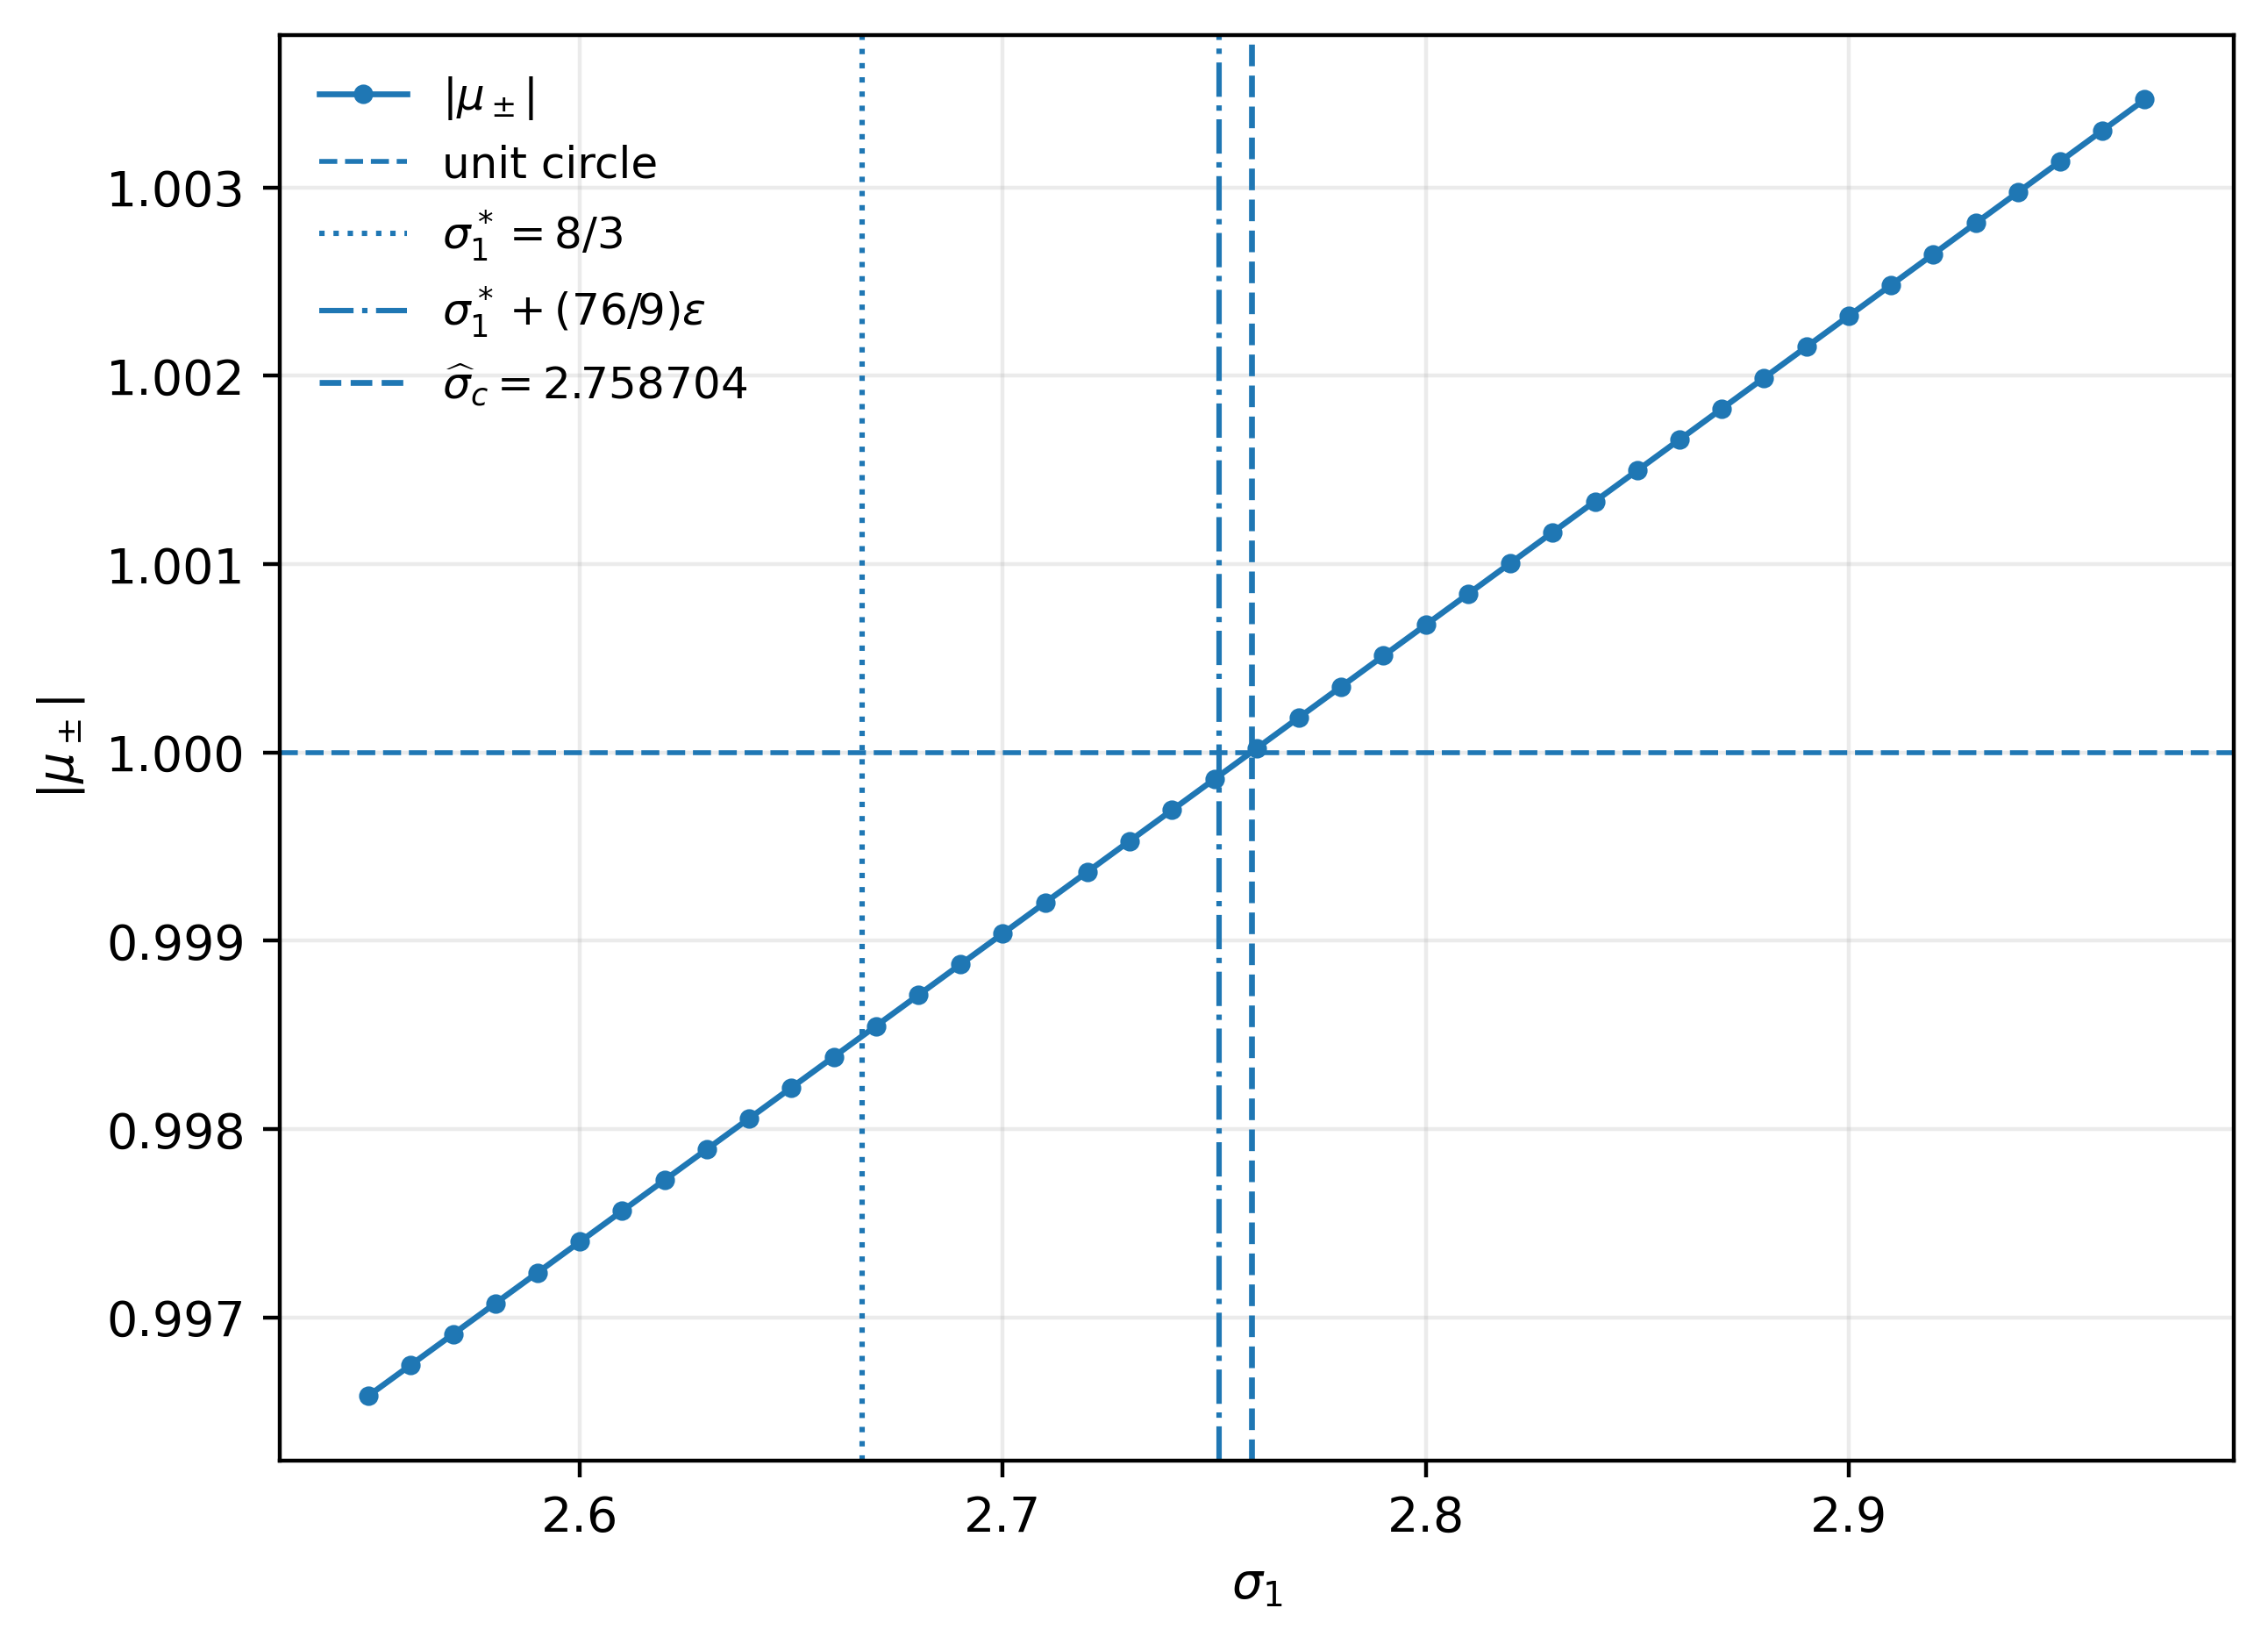
\includegraphics[width=0.82\textwidth]{HR_floquet_crossing_improved.png}
\caption{Full-system Floquet validation for Example~\ref{ex:parameters} at
\(\epsilon=10^{-2}\).  The modulus of the nontrivial conjugate multiplier
pair crosses the unit circle at
\(\widehat{\sigma}_c=2.758704047\ldots\).  The vertical reference lines show
the leading prediction \(\sigma_1^*=8/3\), the first corrected asymptotic
prediction \(\sigma_1^*+(76/9)\epsilon=2.751111\ldots\), and the numerical
crossing.  Throughout the scan the pair remains nonreal; the minimum
absolute imaginary part is \(0.3357\).}
\label{fig:floquet-validation}
\end{figure}

These computations corroborate both the finite-\(\epsilon\) multiplier
crossing and the predicted displacement of the critical parameter.  They
are not part of the proof of Theorem~\ref{thm:NS}; instead, they provide an
independent full-system check of Proposition~\ref{prop:unit-modulus}.  The next subsection complements
this multiplier calculation by displaying the post-bifurcation attracting
set on the canonical Poincar\'e section.


\subsection{Numerical signature of the bifurcating invariant torus}
\label{subsec:torus-validation}

The Floquet calculation locates the loss of transverse stability, but it
does not by itself reveal the geometry of the bifurcating invariant set.
We therefore examine the full system on the parameter side selected by
Theorem~\ref{thm:NS}.  For
\[
 \epsilon=10^{-2},\qquad \sigma_1=2.80,
\]
one has
\[
 \sigma_1-\widehat{\sigma}_c(10^{-2})
 \approx 4.13\times10^{-2}>0.
\]
Since \(\PHR>0\) and \(\LHR<0\) in Example~\ref{ex:parameters},
the theorem predicts a supercritical, normally attracting torus on this
side of the critical curve.

At \(\sigma_1=2.80\), single shooting gives the periodic orbit period
\[
 T=6.198892641\ldots .
\]
The two nontrivial Floquet multipliers are
\[
 \mu_\pm
 =0.935316438\pm0.355721153\,i,
 \qquad
 |\mu_\pm|=1.000676960>1,
\]
so the periodic orbit has already become transversely unstable.

To visualize the nearby attracting set in coordinates consistent with the
analysis, we use the real canonical variables introduced in
Section~2.1.  Let
\[
 \begin{pmatrix}X\\Y\\Z\end{pmatrix}
 =
 P^{-1}
 \begin{pmatrix}u\\v\\w\end{pmatrix},
\]
where \((u,v,w)\) are measured from the fixed equilibrium
\(p_\epsilon\).  The theoretical angular variable satisfies
\(\theta=\operatorname{atan2}(Y,X)\); hence the natural local Poincar\'e
section is
\[
 \Sigma=\{Y=0,\ X>0\}.
\]
On \(\Sigma\) we record
\[
 \rho=\frac{X}{\epsilon},
 \qquad
 \zeta=\frac{Z}{\epsilon}.
\]
The fixed point of this return map corresponding to the unstable periodic
orbit is located numerically at
\[
 (\rho_{\mathrm{po}},\zeta_{\mathrm{po}})
 =(2.025314,-1.444959).
\]

We initialize a trajectory \(10^{-5}\) away from the periodic orbit and
integrate until the section iterates settle onto the attracting set.  A
point on this settled set is then used to restart an independent
high-accuracy DOP853 integration with relative tolerance \(10^{-11}\),
absolute tolerance \(10^{-13}\), and maximum step \(0.2\).  Over
\(1.2\times10^4\) time units, 1938 successive crossings of \(\Sigma\) were
recorded.  As shown in Figure~\ref{fig:torus-section}, these iterates closely
trace a smooth closed curve surrounding the unstable fixed point rather
than collapsing to a finite set.  This is the expected Poincar\'e-section
signature of an invariant two-torus and is consistent with quasiperiodic
motion on that torus.

The numerical rotation number of the closed-curve dynamics, estimated from
the lifted polar angle around the periodic-orbit fixed point, is
\[
 |\varrho_{\mathrm{num}}|\approx 0.0479.
\]
The section points remain on the same closed curve under step-size
refinement and under the independent adaptive integration described above.
Combined with the transverse Floquet instability of the central periodic
orbit and the analytically determined sign \(\LHR<0\), the section provides
a direct full-system corroboration of the supercritical attracting torus
predicted by Theorem~\ref{thm:NS}.  This calculation validates the local
picture; it is not intended as a global continuation of the torus branch.

\begin{figure}[t]
\centering
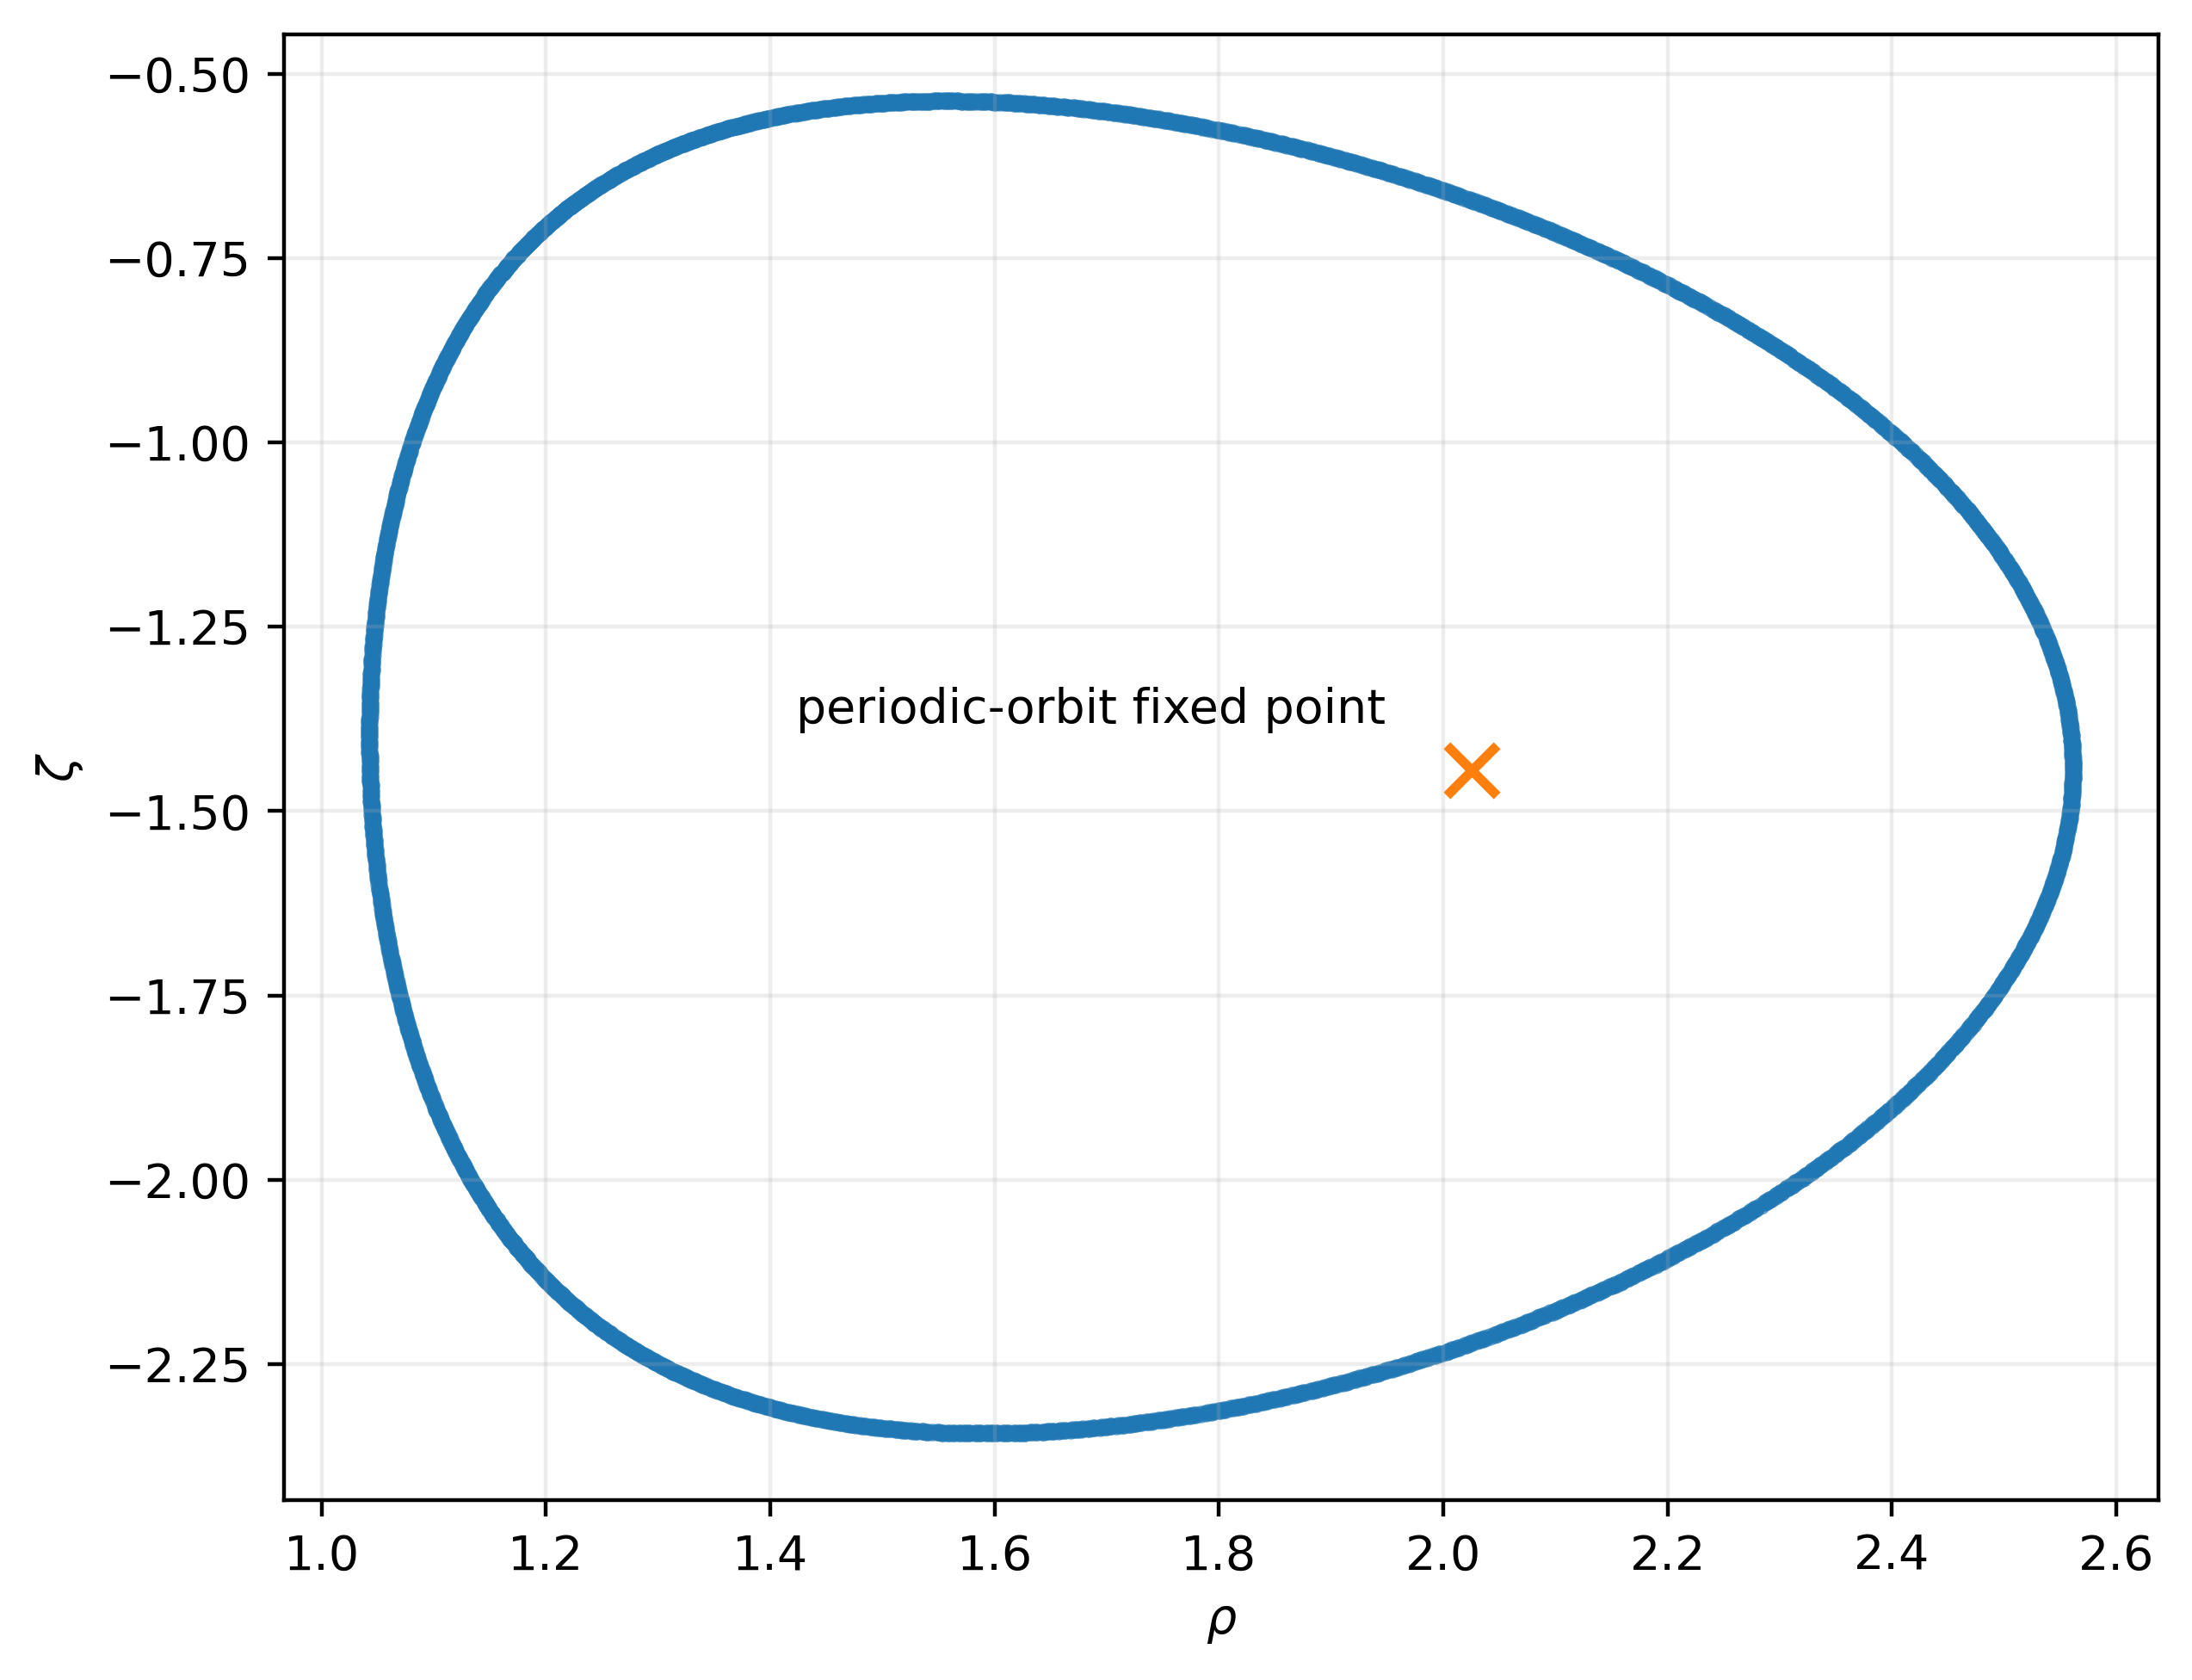
\includegraphics[width=0.78\textwidth]{HR_invariant_torus_poincare_audited.png}
\caption{Canonical Poincar\'e-section signature of the bifurcating invariant
torus for Example~\ref{ex:parameters} with
\(\epsilon=10^{-2}\) and \(\sigma_1=2.80\).
The section is \(\Sigma=\{Y=0,\ X>0\}\), and the plotted coordinates are
\((\rho,\zeta)=(X/\epsilon,Z/\epsilon)\).
The section iterates form a smooth closed curve around the fixed point
(cross) corresponding to the now-unstable periodic orbit.  The 1938 plotted
crossings were obtained from the high-accuracy DOP853 validation run after
the attracting set had been reached.}
\label{fig:torus-section}
\end{figure}


\subsection{Square-root amplitude scaling near the torus bifurcation}
\label{subsec:torus-amplitude-scaling}

The local normal form of a supercritical Neimark--Sacker bifurcation gives
the amplitude law
\[
 R=\mathcal{O}\!\left(
 \sqrt{\sigma_1-\sigma_c(\epsilon)}
 \right)
\]
on the torus-existence side.  The canonical section coordinates \((\rho,\zeta)\) are not the final
normal-form coordinates, but a smooth nonsingular local coordinate change
does not alter the square-root exponent.  This allows us to test the scaling
directly in the full system.

For each value of \(\sigma_1>\widehat{\sigma}_c(10^{-2})\), we compute the
periodic-orbit fixed point
\((\rho_{\rm po},\zeta_{\rm po})\) on the canonical section
\(\Sigma=\{Y=0,\ X>0\}\), allow the post-bifurcation trajectory to settle
onto the attracting closed curve, and define the root-mean-square section
amplitude
\begin{equation}\label{eq:section-amplitude}
 A_\Sigma
 :=
 \left[
 \frac1N\sum_{j=1}^N
 \left(
  (\rho_j-\rho_{\rm po})^2+
  (\zeta_j-\zeta_{\rm po})^2
 \right)
 \right]^{1/2} .
\end{equation}
Table~\ref{tab:torus-amplitude-scaling} lists the resulting amplitudes.

\begin{table}[t]
\centering
\caption{Full-system section amplitude of the attracting invariant curve for
\(\epsilon=10^{-2}\).  Here
\(\Delta\sigma=\sigma_1-\widehat{\sigma}_c\), with
\(\widehat{\sigma}_c=2.758704047\ldots\).}
\label{tab:torus-amplitude-scaling}
\begin{tabular}{cccc}
\hline
\(\sigma_1\) & \(\Delta\sigma\) & \(A_\Sigma\) & \(A_\Sigma^2\)\\
\hline
2.765 & 0.006296 & 0.317482 & 0.100795\\
2.770 & 0.011296 & 0.431217 & 0.185948\\
2.775 & 0.016296 & 0.523868 & 0.274438\\
2.780 & 0.021296 & 0.606541 & 0.367892\\
2.790 & 0.031296 & 0.756850 & 0.572822\\
2.800 & 0.041296 & 0.897794 & 0.806033\\
\hline
\end{tabular}
\end{table}

For the four parameter values closest to the bifurcation, a least-squares
fit of \(A_\Sigma^2\) against \(\sigma_1\) gives
\begin{equation}\label{eq:amplitude-linear-fit}
 A_\Sigma^2
 \approx 17.795603
 \bigl(\sigma_1-2.759448005\bigr),
 \qquad R^2=0.999562.
\end{equation}
The critical parameter inferred solely from the amplitude fit,
\[
 \sigma_c^{\rm amp}=2.759448005,
\]
differs from the independently computed Floquet crossing
\[
 \widehat{\sigma}_c=2.758704047
\]
by only
\[
 \left|\sigma_c^{\rm amp}-\widehat{\sigma}_c\right|
 \approx 7.44\times10^{-4}.
\]
Equivalently, a log--log fit of
\(A_\Sigma=C(\Delta\sigma)^p\) over the same four closest points gives
\[
 p=0.5304,
 \qquad
 R^2=0.999922,
\]
which is close to the Neimark--Sacker normal-form exponent \(1/2\).

Figure~\ref{fig:torus-amplitude-scaling} shows the near-linear dependence
of \(A_\Sigma^2\) on \(\sigma_1\).  The two more distant parameter values are
included to display the onset of higher-order deviations away from the local
bifurcation regime.  Taken together, the Floquet crossing, the attracting invariant closed
curve, and the near-square-root growth of its section amplitude provide
three complementary numerical signatures of the supercritical
Neimark--Sacker bifurcation established analytically in
Theorem~\ref{thm:NS}.

\begin{figure}[t]
\centering
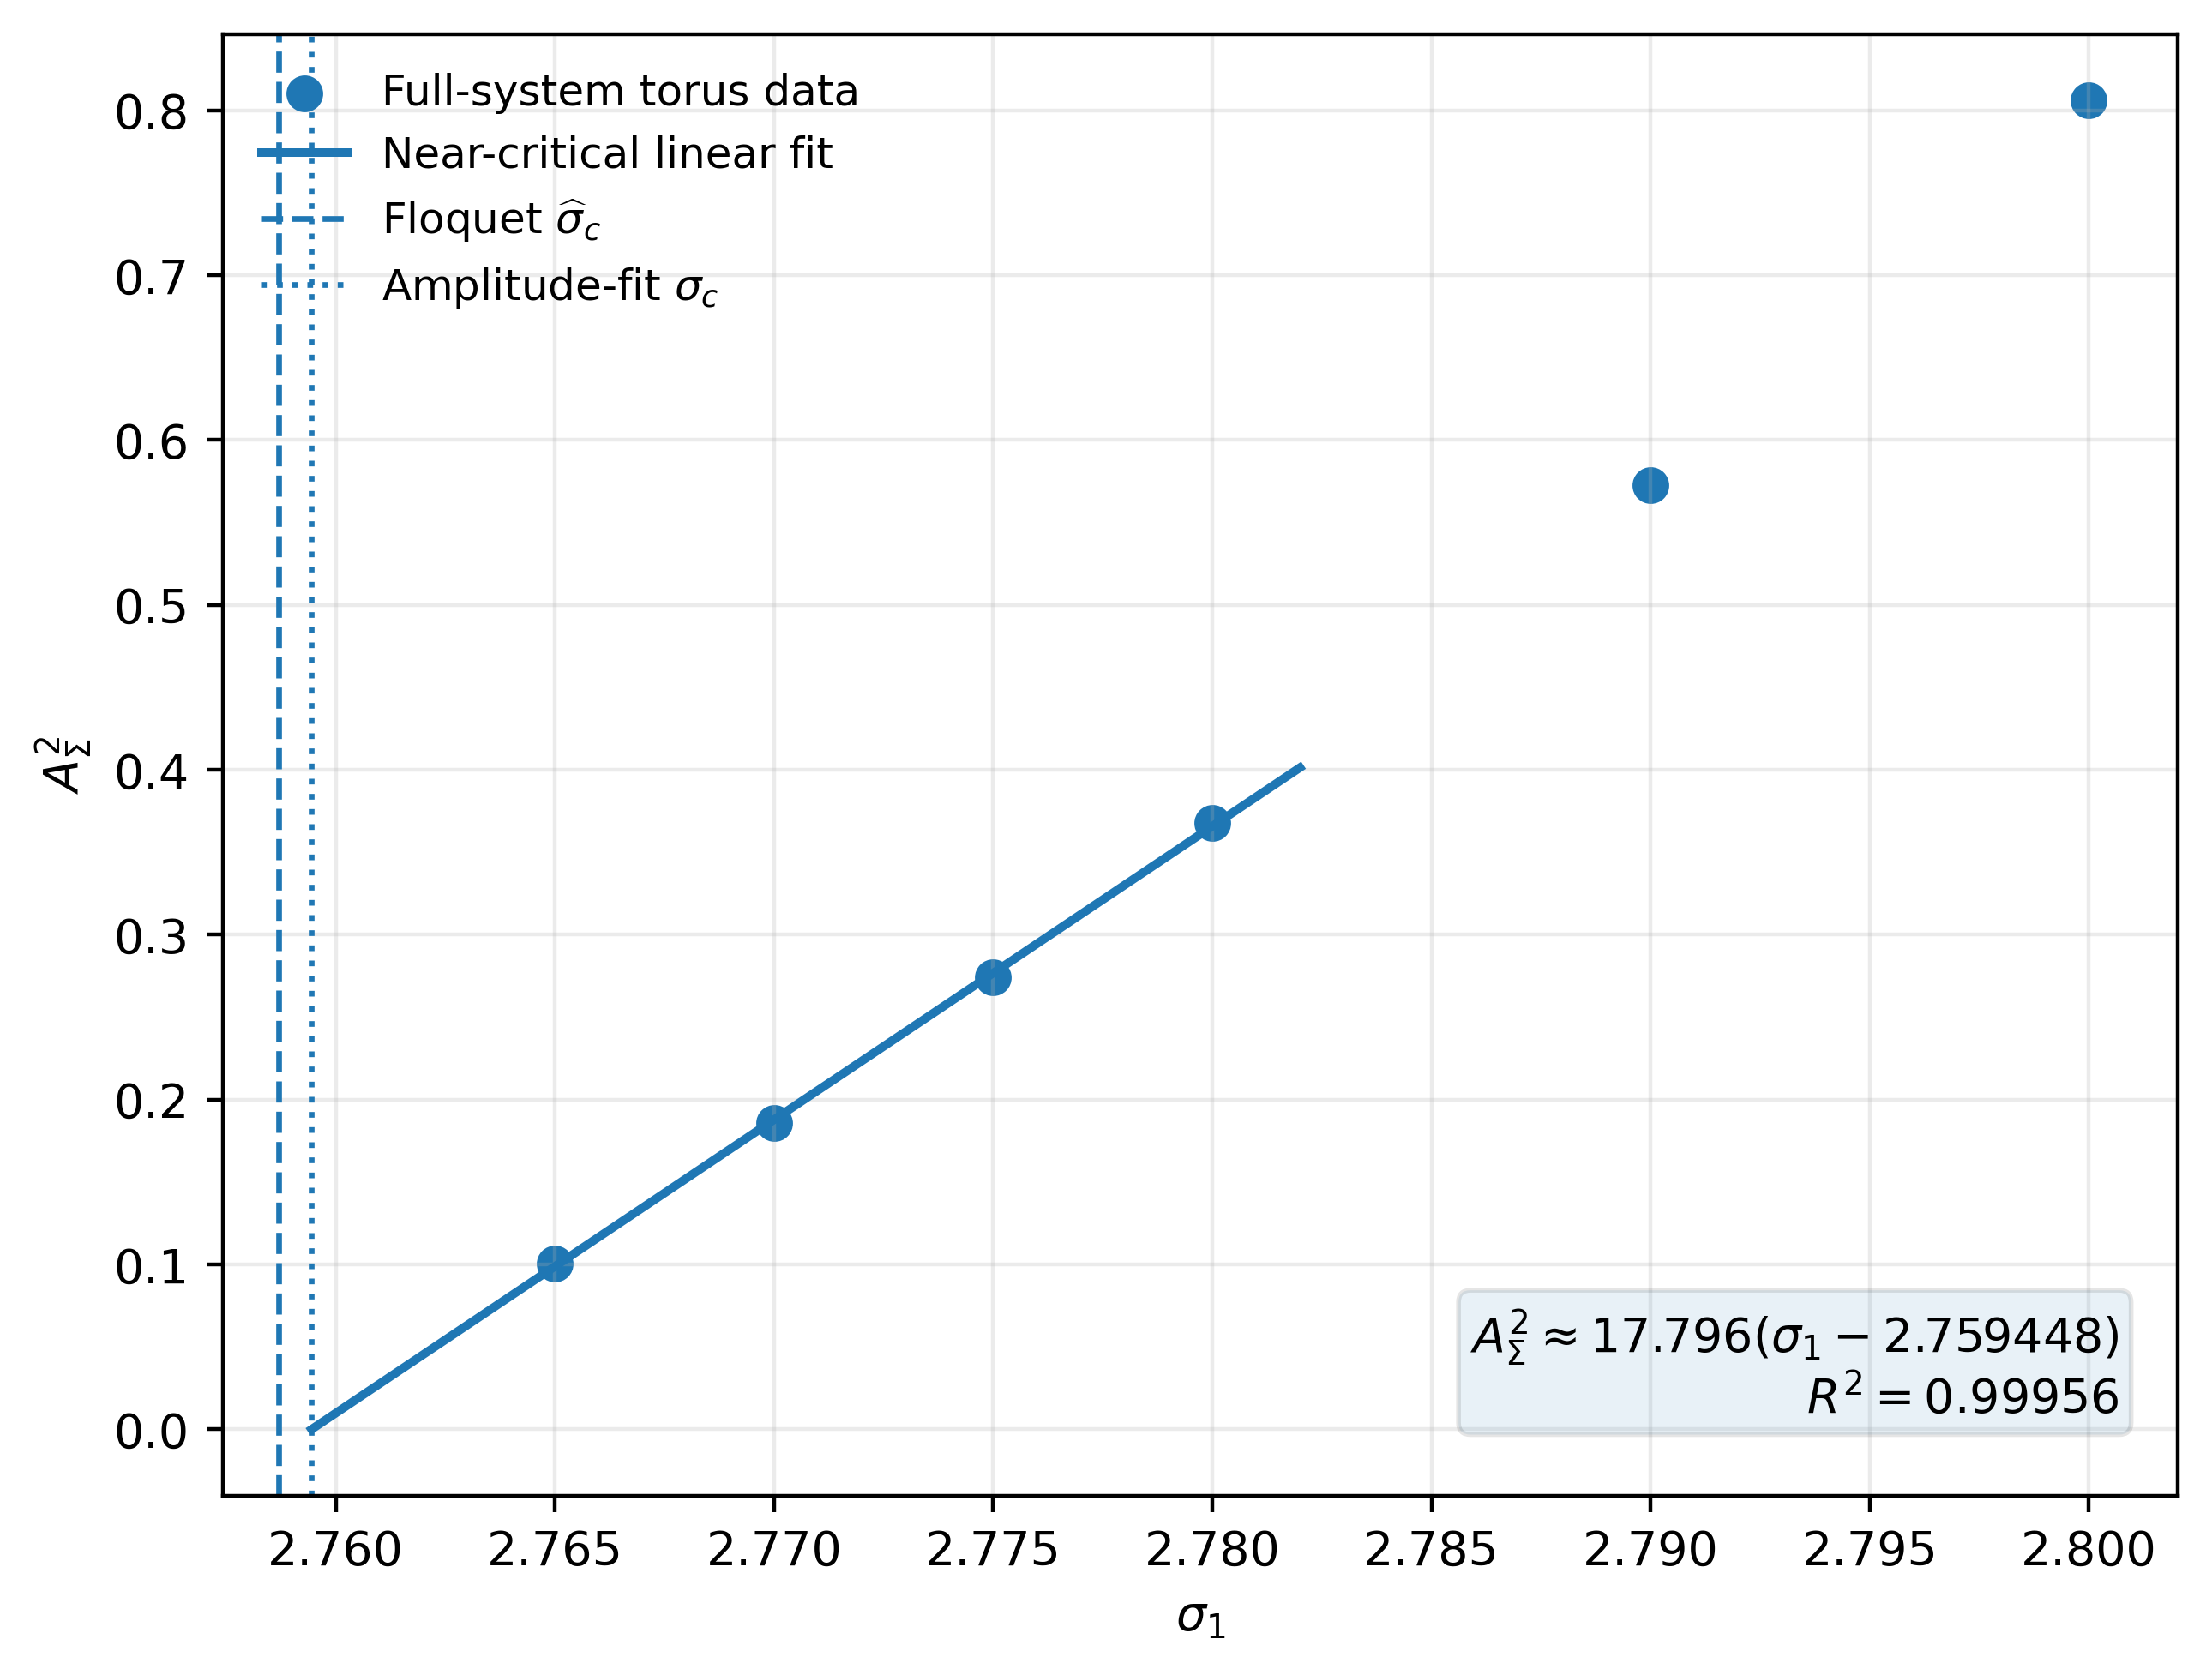
\includegraphics[width=0.78\textwidth]{HR_torus_amplitude_scaling_audited.png}
\caption{Growth of the attracting invariant-curve amplitude on the canonical
Poincar\'e section for \(\epsilon=10^{-2}\).
The ordinate is \(A_\Sigma^2\), defined by
\eqref{eq:section-amplitude}.  The solid line is a linear fit to the four
parameter values closest to the bifurcation.  The vertical dashed line marks
the independently computed Floquet crossing
\(\widehat{\sigma}_c=2.758704047\ldots\), while the dotted line marks the
critical value extrapolated from the amplitude fit.  Their close agreement
and the near-linearity of \(A_\Sigma^2\) are consistent with the expected
square-root torus-amplitude law.}
\label{fig:torus-amplitude-scaling}
\end{figure}


\section{Discussion and conclusions}
\label{sec:discussion}

The analysis carried out in this paper describes a local route from a
zero--Hopf equilibrium to an invariant two-torus in the
Hindmarsh--Rose system. The starting point is the small periodic orbit
created near the zero--Hopf equilibrium, and the main question is what
happens to this orbit when the unfolding parameters are varied. Earlier
work on the HR system established Hopf and zero--Hopf bifurcations and
the corresponding nearby periodic solutions
\cite{BuzziLlibreMedrado2016}. Torus and torus-canard mechanisms have
also been studied in several neuronal models
\cite{BurkeDesrochesBarryKaperKramer2012}, while toroidal behavior in
the HR system has been investigated in stochastic settings
\cite{RyashkoSlepukhina2017,RyashkoSlepukhina2020}. Here we follow the
periodic orbit created near the zero--Hopf point one step further and
show that, under explicit nondegeneracy conditions, it undergoes a
Neimark--Sacker bifurcation that creates a local invariant two-torus.

This mechanism is closely related to the Hopf-zero-to-torus scenario
obtained for the FitzHugh--Nagumo system by C\^andido, Novaes, and
Sadri \cite{candido2027invariant}. In both problems, averaging first
produces a small periodic orbit and the torus is then detected through a
Neimark--Sacker bifurcation of the associated Poincar\'e map. The
present HR calculation, however, makes the finite-$\epsilon$ location of
the bifurcation explicit. The first averaged trace condition identifies
only the leading value $\sigma_1^*$, whereas the actual transverse
multipliers differ from unit modulus at order $\epsilon^2$. Thus the
second-order return map is needed not simply to improve an
approximation, but to determine the true local critical curve
\[
\sigma_c(\epsilon)
=
\sigma_1^*+\epsilon\sigma_{1,1}
+\mathcal{O}(\epsilon^2)
\]
on which the nontrivial Floquet multipliers have exactly unit modulus.
The same calculation also gives the transverse crossing of the unit
circle.

A second feature appears in the normal-form calculation itself. Along
the critical curve, the rotation angle of the Poincar\'e map satisfies
\[
\vartheta_\epsilon=\mathcal{O}(\epsilon),
\]
so the homological resolvents entering the Neimark--Sacker coefficient
become singular as $\epsilon\to0$. This dependence cannot be discarded.
Keeping it throughout the calculation reveals the cancellation of the
nominal order-$\epsilon$ contribution to the first Lyapunov coefficient
and leads to
\[
l_1^\epsilon
=
\epsilon^2L_{\mathrm{HR}}
+\mathcal{O}(\epsilon^3).
\]
The factor $L_{\mathrm{HR}}$ therefore gives the first nonvanishing
criticality coefficient for the unfolding considered here. Because it
can be written explicitly in terms of the HR parameters, its sign
determines whether the bifurcation is supercritical or subcritical and,
accordingly, whether the bifurcating torus is normally attracting or
normally repelling.

The numerical calculations were designed to check these analytical
predictions directly in the full three-dimensional system. They provide
three complementary tests. First, the numerically computed Floquet
crossing approaches the asymptotic critical curve with the predicted
finite-$\epsilon$ displacement. Second, on the parameter side selected
by Theorem~\ref{thm:NS}, the periodic-orbit fixed point on the canonical
Poincar\'e section becomes unstable and is surrounded by an attracting
invariant closed curve. Third, the amplitude of this closed curve grows
approximately as the square root of the distance from the critical
parameter, in agreement with the local Neimark--Sacker normal form.
These computations therefore test the location, geometry, and
criticality of the bifurcation separately. They are intended as
independent full-system checks of the analysis; the existence of the
torus itself follows from the analytical Neimark--Sacker argument.

There are also clear limitations to the result. The most important one
concerns the parameter regime. Under the usual positivity assumptions,
the zero--Hopf relations used here are incompatible with the standard
slow-adaptation HR regime. The theorem should therefore be interpreted
as a rigorous result for the generalized polynomial HR family selected
by the zero--Hopf conditions, rather than as a direct physiological
statement about the conventional neuronal parameter set. The analysis
is also local: it describes the torus close to its birth, but does not
follow it to large amplitude, determine resonance tongues, or describe
torus breakdown and the subsequent transition to more complicated
dynamics. In addition, the numerical validation is carried out for one
explicit algebraic parameter regime. Finally, when
\[
P_{\mathrm{HR}}=0,
\]
the order-$\epsilon^2$ Lyapunov coefficient vanishes, and a higher-order
normal-form calculation would be required.

These limitations point naturally to several directions for further
work. One question is whether a modified HR-type family can realize the
same zero--Hopf-to-torus mechanism while remaining inside a conventional
slow-adaptation parameter regime. A second is to continue the local
torus numerically and investigate how it is connected to resonance
tongues, torus-canard behavior, and torus breakdown. The degenerate case
$P_{\mathrm{HR}}=0$ is another natural problem, since it represents a
higher-codimension situation in which the leading criticality
coefficient no longer determines the local dynamics.

In summary, the local scenario established here is
\[
\begin{aligned}
\text{zero--Hopf equilibrium}
&\;\longrightarrow\;
\text{small periodic orbit}\\
&\;\longrightarrow\;
\text{exact finite-$\epsilon$ unit-modulus crossing}\\
&\;\longrightarrow\;
\text{nondegenerate invariant two-torus}.
\end{aligned}
\]
The main contribution is therefore not the observation of
quasiperiodic behavior in the HR model by itself. Rather, it is the
higher-order analytical construction that identifies where the torus
bifurcation occurs, proves the required nondegeneracy and crossing
conditions, determines the side and normal stability of the bifurcating
torus, and connects these predictions with quantitative computations in
the full system.


\appendix

\section{Exact symbolic verification of the Neimark--Sacker coefficient}

This appendix completes the proof of Lemma~\ref{lem:l1} by deriving the
explicit first Neimark--Sacker Lyapunov coefficient from the second-order
Poincar\'e-map expansion obtained in Section~3.  The calculation is organized
in four steps:
\begin{enumerate}[label=\textup{(\arabic*)},leftmargin=2em]
\item determination of the first correction to the critical fixed point and
to the exact unit-modulus curve;
\item construction of the quadratic and cubic Taylor tensors of the centered
Poincar\'e map;
\item expansion of the homological resolvents appearing in the
Neimark--Sacker normal-form formula;
\item symbolic extraction and simplification of the first Lyapunov
coefficient.
\end{enumerate}
Unless stated otherwise, all quantities in this appendix are evaluated at
the critical point \((q_*,\sigma_1^*)\).

For convenience introduce the notation
\[
 A:=A_*=D_qg_1(q_*;\sigma_1^*),\qquad
 H_1:=D_q^2g_1,\qquad H_2:=D_q^2g_2,\qquad T_2:=D_q^3g_2,
\]
together with
\[
 g_{1,\sigma}:=\partial_{\sigma_1}g_1,\qquad
 A_\sigma:=\partial_{\sigma_1}D_qg_1.
\]
The critical averaged identities established in Section~3 are
\begin{equation}\label{eq:appendix-critical-identities}
\zeta_*=-\frac{A_X}{2B_X},\qquad
\rho_*^2=\frac{A_X^2}{2B_X^2},\qquad
A_Z=\frac{A_XB_Z}{B_X},\qquad
\nu_0^2=-\frac{B_XB_Z\rho_*^2}{\omega^2}.
\end{equation}
Consequently,
\[
 A=\frac{\rho_*}{\omega}
\begin{pmatrix}0&B_X\\B_Z&0\end{pmatrix},
\qquad
A^2=-\nu_0^2I.
\]

\subsection{First correction of the critical fixed point}

The branch of critical fixed points constructed in
Lemma~\ref{lem:fixed-point-branch} has the expansion
\[
 \widehat q_\epsilon=q_*+\epsilon u+\cO(\epsilon^2),
 \qquad u=(u_\rho,u_\zeta)^{\mathsf T}.
\]
Similarly, the exact unit-modulus curve obtained in
Proposition~\ref{prop:unit-modulus} satisfies
\[
 \sigma_c(\epsilon)=\sigma_1^*+\epsilon\sigma_{1,1}+\cO(\epsilon^2).
\]
The unknowns \(u_\rho,u_\zeta,\sigma_{1,1}\) are determined simultaneously by
the order-\(\epsilon\) fixed-point equation together with the
order-\(\epsilon^2\) unit-determinant condition:
\begin{equation}\label{eq:appendix-correction}
 Au+\sigma_{1,1}g_{1,\sigma}+g_2=0,
 \qquad
 \tr A_2+2\pi\det A=0,
\end{equation}
where
\begin{equation}\label{eq:appendix-A2}
 A_2=H_1[u,\cdot]+\sigma_{1,1}A_\sigma+D_qg_2.
\end{equation}
The coefficient matrix of \eqref{eq:appendix-correction} is nonsingular by
Lemma~\ref{lem:fixed-point-branch} together with the transversality condition
\(\tau'(\sigma_1^*)\ne0\).  Hence the system uniquely determines
\((u,\sigma_{1,1})\).  The linear part of the centered Poincar\'e map
therefore has the expansion
\begin{equation}\label{eq:appendix-linear}
 L_\epsilon=I+2\pi\epsilon A+2\pi\epsilon^2A_2+\cO(\epsilon^3).
\end{equation}

\subsection{Quadratic and cubic Taylor tensors}

Since the first averaged function \(g_1\) is quadratic,
\(D_q^3g_1=0\).  Moreover,
\(\partial_{\sigma_1}D_q^2g_1=0\), because the coefficients \(B_X\) and
\(B_Z\) are independent of the bifurcation parameter.  Differentiating the
second-order expansion of the Poincar\'e map therefore gives
\begin{equation}\label{eq:appendix-tensors}
 B_\epsilon=2\pi\epsilon H_1+2\pi\epsilon^2H_2+\cO(\epsilon^3),
 \qquad
 C_\epsilon=2\pi\epsilon^2T_2+\cO(\epsilon^3).
\end{equation}
The displacement \(u\) does not appear explicitly in these tensor
expansions.  Its effect is contained in the linear correction matrix
\(A_2\) and therefore enters the normal-form calculation through the linear
conjugacy.

To transform the linear part into rotation form, write
\[
 \vartheta_\epsilon
=2\pi\nu_0\epsilon+\theta_2\epsilon^2+\cO(\epsilon^3),
\]
where the second-order coefficient \(\theta_2\) is left undetermined.
Introduce
\[
 b_{\mathrm{rot},0}=2\pi A_{12},\qquad
 b_{\mathrm{rot},1}=2\pi(A_2)_{12},
\]
and define
\[
\begin{aligned}
u_S&=\frac{-2\pi^2\nu_0^2-2\pi(A_2)_{11}}{b_{\mathrm{rot},0}},
&
v_0&=-\frac{2\pi\nu_0}{b_{\mathrm{rot},0}},\\
v_1&=-\frac{\theta_2}{b_{\mathrm{rot},0}}
+\frac{2\pi\nu_0b_{\mathrm{rot},1}}{b_{\mathrm{rot},0}^2},
&
S_0&=\begin{pmatrix}1&0\\0&v_0\end{pmatrix},
&
S_1&=\begin{pmatrix}0&0\\u_S&v_1\end{pmatrix}.
\end{aligned}
\]
Let
\[
 T_0=S_0^{-1},\qquad
 T_1=
\begin{pmatrix}
0&0\\
-u_S/v_0&-v_1/v_0^2
\end{pmatrix}.
\]
Expansion of the exact conjugacy matrix in
\eqref{eq:rotation-conjugacy} gives
\[
 S_\epsilon=S_0+\epsilon S_1+\cO(\epsilon^2),
 \qquad
 S_\epsilon^{-1}=T_0+\epsilon T_1+\cO(\epsilon^2).
\]
For vectors \(x,y,z\in\mathbb{C}^2\), define
\[
 U_1(x,y)=2\pi H_1[x,y],\qquad
 U_2(x,y)=2\pi H_2[x,y],\qquad
 V_2(x,y,z)=2\pi T_2[x,y,z].
\]
Substitution into the transformation formulas for multilinear tensors yields
\begin{equation}\label{eq:appendix-transformed-tensors}
\widetilde B_\epsilon
=\epsilon B_0+\epsilon^2B_1+\cO(\epsilon^3),
\qquad
\widetilde C_\epsilon
=\epsilon^2C_0+\cO(\epsilon^3),
\end{equation}
where
\[
\begin{aligned}
B_0(x,y)
&=T_0U_1(S_0x,S_0y),\\
B_1(x,y)
&=T_1U_1(S_0x,S_0y)
+T_0U_1(S_1x,S_0y)
+T_0U_1(S_0x,S_1y)
+T_0U_2(S_0x,S_0y),\\
C_0(x,y,z)
&=T_0V_2(S_0x,S_0y,S_0z).
\end{aligned}
\]
Equations \eqref{eq:appendix-correction},
\eqref{eq:appendix-linear}, and \eqref{eq:appendix-transformed-tensors}
contain every quantity that contributes to the first Lyapunov coefficient
through order \(\epsilon^2\).

\subsection{Homological resolvents}

Let
\[
 q=\begin{pmatrix}1\\-i\end{pmatrix},
 \qquad
 p_{\mathrm{ad}}=\frac12\begin{pmatrix}1\\-i\end{pmatrix}.
\]
The linear part of the centered map is the rotation
\(R_{\vartheta_\epsilon}\), whose angle satisfies
\[
 \vartheta_\epsilon=2\pi\nu_0\epsilon+\theta_2\epsilon^2+\cO(\epsilon^3).
\]
Accordingly,
\[
 R_{\vartheta_\epsilon}=I+\epsilon J_1+\epsilon^2R_2+\cO(\epsilon^3),
\]
where
\[
 J_1=
\begin{pmatrix}
0&-2\pi\nu_0\\
2\pi\nu_0&0
\end{pmatrix},
\qquad
 R_2=
\begin{pmatrix}
-2\pi^2\nu_0^2&-\theta_2\\
\theta_2&-2\pi^2\nu_0^2
\end{pmatrix}.
\]
The homological equations defining the normal-form transformation are
\[
 (I-R_{\vartheta_\epsilon})h_{11}
=\widetilde B_\epsilon(q,\overline q),
\qquad
 (\lambda_\epsilon^2I-R_{\vartheta_\epsilon})h_{20}
=\widetilde B_\epsilon(q,q).
\]
Although the corresponding linear operators become singular as
\(\epsilon\to0\), the singularity is exactly compensated by the fact that
\(\widetilde B_\epsilon=\cO(\epsilon)\).  Consequently both homological
vectors admit finite asymptotic expansions
\[
 h_{11}=h_{11}^{(0)}+\epsilon h_{11}^{(1)}+\cO(\epsilon^2),
 \qquad
 h_{20}=h_{20}^{(0)}+\epsilon h_{20}^{(1)}+\cO(\epsilon^2).
\]
Substituting the tensor expansions above gives
\[
\begin{aligned}
h_{11}^{(0)}
&=(-J_1)^{-1}B_0(q,\overline q),\\
h_{11}^{(1)}
&=(-J_1)^{-1}\bigl(B_1(q,\overline q)+R_2h_{11}^{(0)}\bigr),\\
h_{20}^{(0)}
&=N_1^{-1}B_0(q,q),\\
h_{20}^{(1)}
&=N_1^{-1}\bigl(B_1(q,q)-N_2h_{20}^{(0)}\bigr),
\end{aligned}
\]
where
\[
 N_1=4\pi i\nu_0I-J_1,
\qquad
 N_2=(2i\theta_2-8\pi^2\nu_0^2)I-R_2.
\]
Since \(\nu_0>0\), both \(-J_1\) and \(N_1\) are nonsingular.

\subsection{Symbolic extraction of the first Lyapunov coefficient}

Define
\[
\begin{aligned}
\mathfrak N_1
&=2B_0(q,h_{11}^{(0)})
+B_0(\overline q,h_{20}^{(0)}),\\
\mathfrak N_2
&=C_0(q,q,\overline q)
+2B_0(q,h_{11}^{(1)})+2B_1(q,h_{11}^{(0)})\\
&\quad+B_0(\overline q,h_{20}^{(1)})
+B_1(\overline q,h_{20}^{(0)}).
\end{aligned}
\]
Substitution into the exact Neimark--Sacker coefficient formula
\eqref{eq:l1-formula} gives
\[
 l_1^\epsilon
=\epsilon\ell_{1,1}+\epsilon^2\ell_{1,2}+\cO(\epsilon^3),
\]
where
\[
 \ell_{1,1}=\frac12\operatorname{Re}
\langle p_{\mathrm{ad}},\mathfrak N_1\rangle,
\]
and
\[
 \ell_{1,2}
=\frac12\operatorname{Re}\left(
\langle p_{\mathrm{ad}},\mathfrak N_2\rangle
-2\pi i\nu_0\langle p_{\mathrm{ad}},\mathfrak N_1\rangle
\right).
\]

The order-\(\epsilon\) cancellation can be shown explicitly, rather than
left as an opaque computer-algebra simplification.  Set
\[
 \chi:=v_0=-\frac{2\pi\nu_0}{b_{\mathrm{rot},0}}.
\]
Since \(b_{\mathrm{rot},0}=2\pi\rho_*B_X/\omega\), the critical identities give
\[
 \chi^2=-\frac{B_Z}{B_X},
 \qquad
 \nu_0=-\frac{\rho_*B_X}{\omega}\chi.
\]
Using \(S_0=\operatorname{diag}(1,\chi)\) in the definition of \(B_0\) gives
\[
 B_0(q,\overline q)
 =
 \begin{pmatrix}
 0\\[1mm]
 -\dfrac{2\pi B_X\chi}{\omega}(2\chi^2+1)
 \end{pmatrix},
\]
and
\[
 B_0(q,q)
 =
 \begin{pmatrix}
 -\dfrac{4\pi i B_X\chi}{\omega}\\[1mm]
 \dfrac{2\pi B_X\chi}{\omega}(2\chi^2-1)
 \end{pmatrix}.
\]
The leading homological vectors are therefore
\[
 h_{11}^{(0)}
 =
 \begin{pmatrix}
 -\dfrac{2\chi^2+1}{\rho_*}\\[1mm]0
 \end{pmatrix},
 \qquad
 h_{20}^{(0)}
 =
 \begin{pmatrix}
 \dfrac{5-2\chi^2}{3\rho_*}\\[2mm]
 \dfrac{4i(\chi^2-1)}{3\rho_*}
 \end{pmatrix}.
\]
A direct substitution then yields
\begin{equation}\label{eq:leading-cancellation}
 \left\langle p_{\mathrm{ad}},\mathfrak N_1\right\rangle
 =
 \frac{4\pi iB_X\chi}{3\rho_*\omega}
 \left(2\chi^4+5\chi^2+2\right).
\end{equation}
The right-hand side is purely imaginary because
\(B_X,\chi,\rho_*,\omega\in\mathbb{R}\).  Hence
\[
 \boxed{\ell_{1,1}=0}.
\]
Thus the first nonzero contribution can occur only at order
\(\epsilon^2\).

For the order-\(\epsilon^2\) coefficient, substitute the polynomial
expressions \eqref{eq:G21}--\eqref{eq:G22} into
\(H_2=D_q^2g_2\) and \(T_2=D_q^3g_2\), solve
\eqref{eq:appendix-correction} for
\((u_\rho,u_\zeta,\sigma_{1,1})\), and insert the resulting
\(A_2,B_1,C_0,h_{11}^{(1)},h_{20}^{(1)}\) into
\(\mathfrak N_2\).  Simplification with the critical identities
\eqref{eq:appendix-critical-identities} eliminates the auxiliary quantities
\[
 C_X,C_Y,C_Z,\quad D_X,D_Y,D_Z,\quad E_Y,E_Z,\quad
 \sigma_{1,1},\quad \theta_2,
\]
and leaves a coefficient depending only on
\(B_X,B_Y,B_Z,E_X,\omega\):
\begin{equation}\label{eq:appendix-coefficients}
\ell_{1,1}=0,\qquad
\ell_{1,2}
=-\frac{\pi B_Z(B_X+B_Z)}{2B_X^2\omega^2}
\bigl(2B_XB_Y-7B_YB_Z-3E_X\omega\bigr).
\end{equation}
Consequently,
\[
 l_1^\epsilon=\epsilon^2\LHR+\cO(\epsilon^3),
\]
where \(\LHR\) is exactly \eqref{eq:LHR-averaged}.

Two features of this reduction are important.  First,
\(\ell_{1,1}=0\) is a structural cancellation of the leading quadratic
normal-form contribution, as \eqref{eq:leading-cancellation} shows; it is not
a numerical coincidence.  Second, \(\ell_{1,2}\) is independent of
\(\beta_2\) and \(\sigma_2\) because the second-order unfolding coefficients
contained in \(C_X,C_Y,C_Z\) cancel from the final expression.

\subsection{Reduction to the Hindmarsh--Rose parameters}

Substituting
\[
 B_X=\frac{D_0}{\omega^2},\qquad
 B_Y=\frac{d-(1+r)k_0}{\omega},\qquad
 B_Z=\frac{r(k_0-d)}{\omega^2},\qquad
 E_X=-\frac{a(\omega^2-r)}{\omega^2}
\]
into \eqref{eq:appendix-coefficients}, and using
\[
 D_0+r(k_0-d)=k_0\omega^2,
\]
gives
\[
\LHR
=-\frac{\pi k_0r(k_0-d)}{2\omega^3D_0^2}
\left[
3a\omega^2(\omega^2-r)
+\bigl(2k_0\omega^2+9r(d-k_0)\bigr)
\bigl(d-k_0(1+r)\bigr)
\right].
\]
This is exactly the factorized formula \eqref{eq:LHR-factorized}.

\begin{remark}[Reproducibility]\label{rem:reproducibility}
The accompanying symbolic-verification script uses exact SymPy arithmetic
for three complementary checks.  First, before any specialization to an HR
parameter set, it verifies the structural cancellation
\(\ell_{1,1}=0\) in \eqref{eq:leading-cancellation}.  Second, it reconstructs
the complete order-\(\epsilon^2\) normal-form calculation for
Example~\ref{ex:parameters}, including
\(\sigma_{1,1}=76/9\), and obtains
\[
 \ell_{1,2}=-\frac{2016\pi}{121};
\]
Third, it verifies identically the algebraic reduction from
\eqref{eq:LHR-averaged} to \eqref{eq:LHR-factorized}.  The full-system
shooting and variational calculations in Section~4 are independent of these
symbolic checks.

These scripts serve as reproducibility and error-detection tools.  The proof
remains the analytical expansion given above; in particular, neither the
uniform remainder estimates nor the application of the
Neimark--Sacker theorem is delegated to computer algebra.
\end{remark}

\bibliographystyle{amsplain}
\bibliography{bibliography_step9_doi}

\end{document}
